\chapter{\acf{camion}}

\section{Motivation}

Uneven distributions of population and health-care providers lead to geographic
disparity in accessibility for patients \cite{wang_why_2020}, illustrated by our
previous results on accessibility. Several methods have been developed to
address these disparities. Location-allocation algorithms
\cite{church_location_1999} can optimize the distribution and supply of health
providers to reduce accessibility disparities. These algorithms seek the optimal
placement of facilities for a desirable objective under certain constraints
\cite{wang_measurement_2012}. For instance, Luo et al. developed an optimization
algorithm to improve the healthcare planning in rural China by finding the best
place and capacity for new health facilities \cite{luo_integrating_2014}. Tao et
al. worked on a spatial optimization model to maximize equity in accessibility
to residential care facility in Beijing, China \cite{tao_spatial_2014}. When
optimizing health accessibility, there are two competing goals: equity and
efficiency \cite{krugman_opinion_2013,meyer_equity_2008}. Equity may be defined
as equal access to healthcare for everyone \cite{culyer_equity_1993}. An
efficient situation is when everything has been done to help any person without
harming anyone else \cite{hemenway_optimal_1982}. While some argue that
efficiency should be ad-dressed in priority \cite{hemenway_optimal_1982}, others
agree that equity is a matter of ethical obligation, especially in public health
\cite{fried_rights_1975, oliver_equity_2004}. Regarding efficiency optimization,
the most popular algorithms are p-median, \ac{lscp} and \ac{mclp}. The p-median
algorithm minimizes the weighted sum of distances between users and facilities
\cite{murad_using_2021}. \ac{lscp} minimizes the number of facilities needed to
cover all demand \cite{shavandi_fuzzy_2006}. \ac{lscp} maximizes the demand
covered within a desired distance or time threshold by locating a given number
of facilities \cite{casado_heuristical_2005}. To reach equal access to
healthcare, quadratic programming has been used to  minimize the variance of
accessibility scores defined by the \ac{2sfca} \cite{wang_planning_2013}.
Similarly, a \ac{pso} algorithm was developed to minimize the total square
difference between the accessibility score of each demand location and the
weighted average accessibility score \cite{tao_spatial_2014}. Finally, a
two-step optimization algorithm has been developed to address the dual
objectives of efficiency and equality, by first choosing where to site new
hospitals and then deciding which capacity they should have
\cite{luo_two-step_2017,li_two-step_2017}.

However, most of the previous algorithms seek locations to open new health
facilities. Regarding oncology care, opening new facilities can be very costly
and hard in practice. In this work, we are interested in the case where the
health facilities locations are fixed, and the only lever to improve
accessibility is to increase their capacities.Given a capacity budget, we want
to know which facilities to grow and by how much. We introduce \ac{camion}, an
accessibility optimization algorithm based on \ac{fca} and \ac{lp}. The initial
accessibility score was computed with the \ac{e2sfca} algorithm
\cite{luo_enhanced_2009} but our algorithm can generalize to more \ac{fca}
derivatives. In the following sections, we proposed two approaches for
optimizing the accessibility scores. The first one is an overall optimization,
where we seek to maximize the total accessibility. The second one is a maxi-min
optimization, where we want to maximize the minimum accessibility instead. The
first approach could be seen as efficiency maximization where the second method
aims towards equity. Then, we embedded our results and algorithms into a
web application  called ``oncology-accessibility''. Through this web
application, we let the users run the optimization algorithm with the
parameters they want, and visualize the output on interactive maps and
figures. We believe such an app could benefit the healthcare professionals,
to help addressing the accessibility disparities in the country.

\section{Methods}

\subsection{Overall optimization}

We model the problem as an optimization task. In our case, we want our
optimization algorithm to find new care centers capacities given some
constraints, so that the total accessibility is maximum. We apply optimization
on a given region only, rather than on the whole metropolitan France. We chose
this approach because healthcare planning is handled regionally rather than
nationally. We show below that our optimization problem is a \acf{lp} problem. In
its standard form, \ac{lp} finds a vector $x$ that maximizes $c^T x$ under
constraints $Ax \leq b$, where $A$ is a matrix and $b$ a vector. Boundaries can
be set to $x$ such as $x \geq 0$. Consider $x_u$ the new capacity of a care
center $u$, to be computed by the algorithm. Let $Q_u$ and $W_u$ be two vectors
of size $m$, defined as follows:

\begin{align}
    Q_u & =  \sum_{s=1}^{r} W_s \sum_{i, d_{iu} \in I_s} P_i \\[10pt]
    W_u & =  \sum_{s=1}^{r} \sum_{i, d_{iu} \in I_s} W_s
\end{align}

Intuitively, $Q_u$ is the weighted population that has access to the care center
$u$, and $W_u$ is the sum of weights of municipalities that have access to $u$.
We can compute the total accessibility as a sum on the $m$ care centers:

\begin{align*}
    \sum_{i} A_i & = \sum_{i} \sum_{s=1}^{r} W_s \sum_{u, d_{iu} \in I_s} \frac{S_u}{Q_u} \\[10pt]
    \sum_{i} A_i & = \sum_{i} \sum_{i, d_{iu} \in I_s} W_s \frac{S_u}{Q_u}                \\[10pt]
    \sum_{i} A_i & = \sum_{u} \frac{S_u}{Q_u} \sum_{s} \sum_{i, d_{iu}} W_s               \\[10pt]
    \sum_{i} A_i & = \sum_{u} \frac{S_u}{Q_u} W_u \numberthis \label{eq:A_i_sum_u}
\end{align*}

\cref{eq:A_i_sum_u} can be rewritten in the \ac{lp} standard form with:

\begin{align*}
    c                & = \frac{W_u}{Q_u}              \\
    x_u              & = S_u                          \\
    b                & \geq \sum_{u} x_u              \\
    x_{u_\text{min}} & \leq x_u \leq x_{u_\text{max}}
\end{align*}

The user-defined parameters are $b$, $x_{u_\text{min}}$ and $x_{u_\text{max}}$.
$b$ is the total capacity to be shared across all the care centers.
$x_{u_\text{min}}$ and $x_{u_\text{max}}$ are the capacity boundaries for care
center $u$. If $b$ is set to the current total capacity, a care center can’t be
grown unless another one is decreased. If $b > \sum_{u} x_u$, the capacity of
care centers can be increased without decreasing other centers. We know how to
solve \ac{lp} and we used the SciPy \cite{virtanen_scipy_2020} implementation of
the revised simplex method as explained in \cite{bertsimas_introduction_1998}.
We now detail how we set the user-defined parameters to apply the \ac{lp}
algorithm to our specific case. The additional capacity was set as +3\% of the
overall activity of the region's care centers: $b = 1.03 \times \sum_{u} x_u$.
The choice of the boundaries $x_{u_\text{min}}$  and $x_{u_\text{max}}$ is
crucial and must be realistic. We studied the hospitals activity on the past
four years (2016 to 2019) to retrieve the average growth percentage of a care
center. The growth percentage is computed as follows: $(S_\text{2019} -
    S_\text{2016}) / S_\text{2016}$ . Among the care centers that grew and who had
an existing oncology activity, the mean growth percentage was 23\%. Hence, we
set $x_{u_\text{max}}$ as +20\% of the care center capacity. Regarding
$x_{u_\text{min}}$, we set the boundary based on the cluster of the care center.
For the three most specialized clusters, we set their $x_{u_\text{min}}$ equal
to their current activity. We did this to prevent the algorithm from decreasing
the most specialized and well-equipped care centers. Regarding the care centers
from the other clusters, $x_{u_\text{min}}$, so that they could be emptied if
need be. Finally, we set $x_{u_\text{max}}$ if the care center belongs to the
least specialized cluster. The new capacities are indicative and should be
further investigated to make sure they are relevant. Especially when setting an
existing oncology activity to 0.

\subsection{Maxi-min optimization}

We now want to maximize the minimum accessibility, meaning that the facilities
capacities will be increased to develop the areas where the accessibility is
minimum in priority. Let $z$ be the minimum accessibility score.

\begin{align}
    z & = \underset{i=1, ..., n}{min} A_i       \\
    z & \leq A_i \; \text{for all} \; i=1,...,n
    \label{eq:z-inequality}
\end{align}

Let $x_u$ be the capacity increase for facility $u$,
whose current capacity was $S_u$. A facility with an unchanged capacity will
have $x_u=0$. The accessibility score $A_i$ at municipality $i$ computed with the
\ac{e2sfca} algorithm can be written as:

\begin{align*}
    A_i & = \sum_{s=1}^{r} W_s \sum_{u,d_{iu} \in I_s} \frac{S_u + x_u}{Q_u}
    \label{eq:A_i}
\end{align*}

Replacing $A_i$ with this previous formulation in \cref{eq:z-inequality} brings
the following:

For all $i=1, ... ,n$:

\begin{align*}
    z                                                              & \leq \sum_{s=1}^{r} W_s \sum_{u, d_{iu} \in I_s} \frac{S_u + x_u}{Q_u} \\
    z - \sum_{s=1}^{r} W_s \sum_{u,d_{iu} \in I_s} \frac{x_u}{Q_u} & \leq \sum_{s=1}^{r} W_s \sum_{u,d_{iu} \in I_s} \frac{S_u}{Q_u}
\end{align*}

We can add these new $n$ equations as constraints to the optimization problem,
as well as the other constraints. The Linear Programming problem is now framed
as the maximization of $c^T x$ with $c=(1, ... ,0)$ and $x=(z, ... ,0)$, both of
size $m+1$ with m the number of facilities. The constraints are:

For all $i=1, ... ,n$:

\begin{align*}
    z - \sum_{s=1}^{r} W_s \sum_{u,d_{iu} \in I_s} \frac{x_u}{Q_u} & \leq \sum_{s=1}^{r} W_s \sum_{u,d_{iu} \in I_s} \frac{S_u}{Q_u} \\
    \sum_{u} x_u                                                   & \leq b \; \text{for a given budget} \; b                        \\
    x_{u_\text{min}}                                               & \leq x_u \leq x_{u_\text{max}}
\end{align*}

\section{Results}

We now present the outcomes of our optimization algorithm, on every region in
metropolitan France. We chose to run the overall optimization approach, because
it led to better results. Indeed, with the maxi-min approach, the municipalities
with low population densities and few hospitals were targeted first. Since these
municipalities often have access to non specialized hospitals, the only lever we
had was to develop these smaller hospitals, which could be very costly. The
algorithm was ran on every region and the additional number of stays was set to
3\% of the current region's overall activity and capped care centers to a
20\% maximum growth.

\subsection*{Provence Alpes Cote d'Azur}

We allocated 3,221 new stays in this region, corresponding to 3\% of the overall
activity. The median accessibility in the region went from 0.0093 to 0.0103, a
11.1\% increase. The results are shown on \cref{fig:optim-paca}. Map (A)
displays the accessibility delta ($A_{i_\text{after}} - A_{i_\text{before}}$) as
well as the care centers eligible to grow. Centers from cluster 8 were hidden
since we considered that they couldn't provide any oncology activity. The
algorithm identified a list of 26 care centers where the oncology activity could
grow to maximize the total accessibility in the region. These centers are either
public or private hospitals, primarily located in the Avignon and Gap areas. The
care centers located in high accessibility areas near Marseille and Nice were
ignored by the algorithm because improving these zones is not a priority. The
care center that grew the most is Clinique Sainte Catherine, in Avignon.
Interestingly, this care center was recently bought by the Unicancer group,
which coordinates all the cancer centers in France. This hospital's type will
change to become a new \ac{clcc}. Thus, it is expected to grow in the next years
and to be equipped with more oncology services and staff.

\begin{figure}[H]
    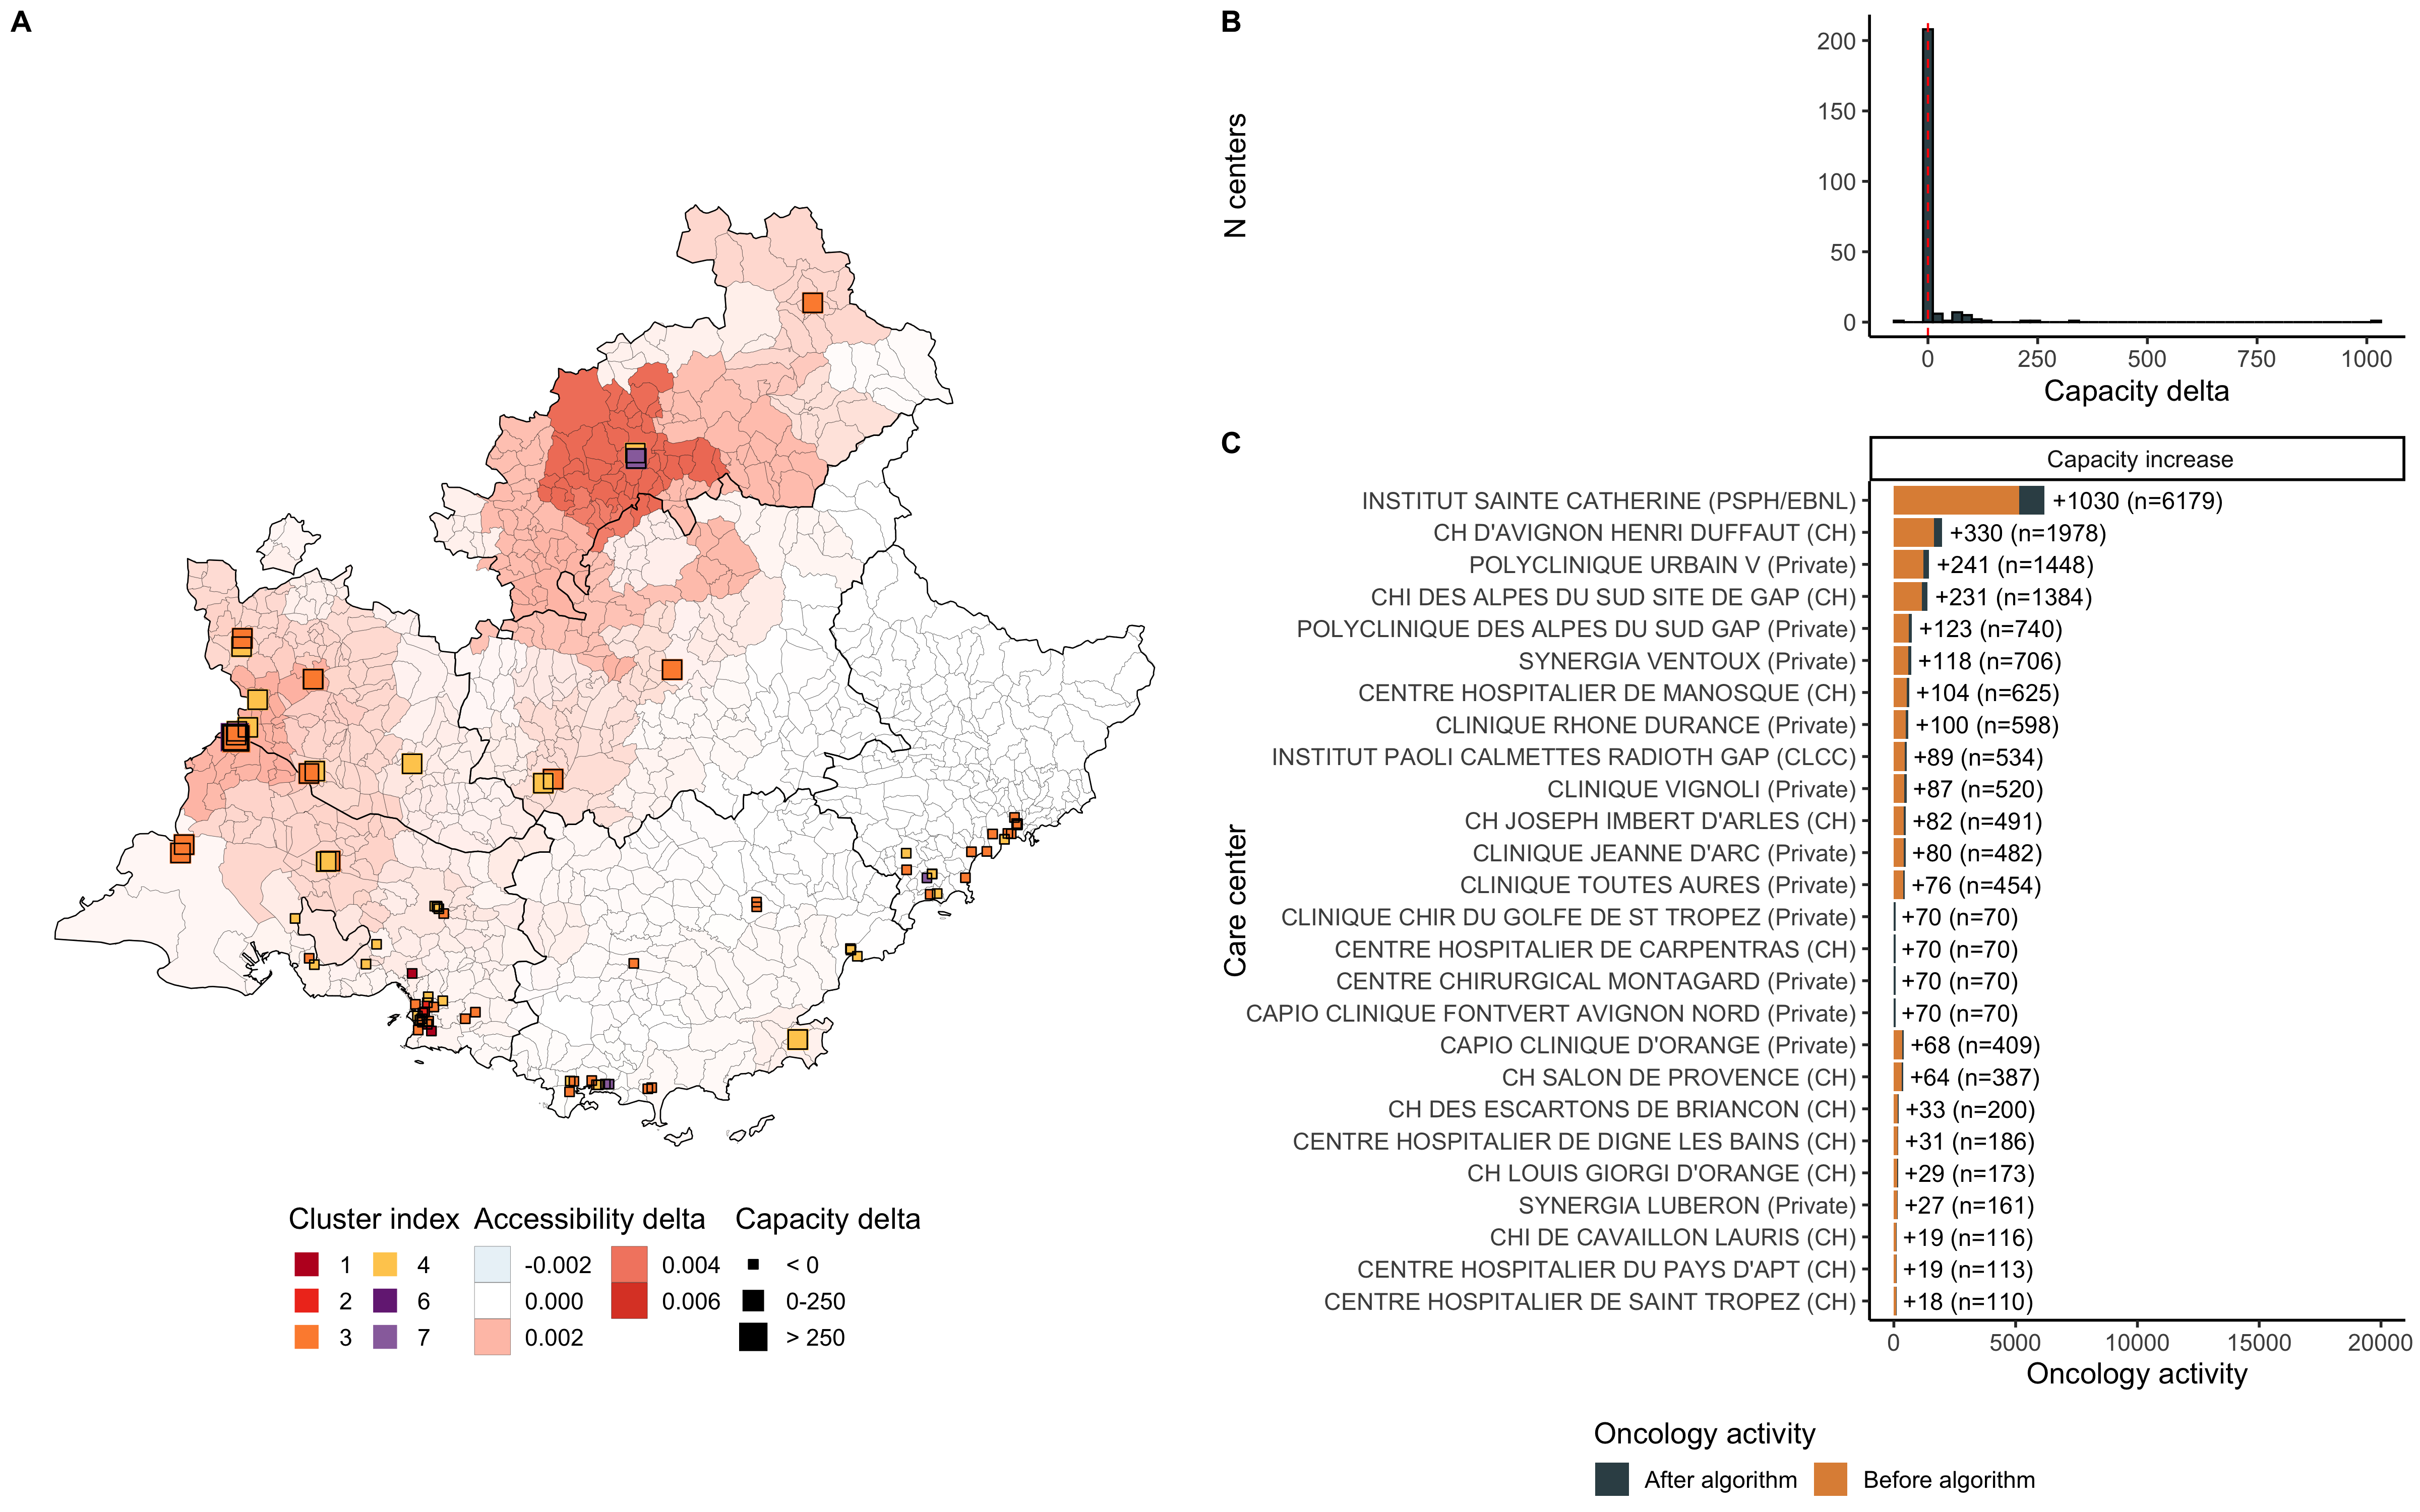
\includegraphics[width=0.9\textwidth]{images/camion/fig5_Provence-Alpes-Cote-d'Azur.png}
    \centering
    \caption{ \textbf{Accessibility delta in Provence-Alpes-Cote-d'Azur region
        after running the optimization algorithm.} Map (A) displays the
    accessibility delta ($A_{i_\text{after}} - A_{i_\text{before}}$) by
    municipality. Plot (B) shows the capacity delta
    ($S_{u_\text{after}}-S_{u_\text{before}}$) distribution. Capacity was
    defined as the oncology activity: the number of patients with
    chemotherapy or radiotherapy and the number of medical or surgery stays
    related to oncology. We show the list of the care centers that grew the
    most (C)  and by how much. For instance, the hospital Institut Sainte
    Catherine in Avignon, was assigned a +1,030 capacity, for a total of
    n=6,179. Additional activity was 3,221. 26 centers grew and 1 decreased.
    Median accessibility before optimization was 0.0093 and 0.0103 after,
    corresponding to a 11.1\% increase.  Accessibility increased around
    cities like Avignon and Gap. Care centers near Nice were left unchanged
    by the algorithm. }
    \label{fig:optim-paca}
\end{figure}

\subsection*{Pays de la Loire}

Similarly, we describe the optimization results in the Pays-de-la-Loire region,
obtained with the same parameters for the algorithm. The additional activity was
1,890. A total of 18 centers grew and 2 were decreased. The median accessibility
before optimization was 0.0118 and 0.0121 after, corresponding to a 2.4\%
increase. Accessibility mainly grew near Le Mans, Angers and La Roche sur Yon.
The three hospitals that had the highest increase in capacity were \ac{ch}
du Mans, a public hospital; Clinique Victor Hugo, a private hospital; and
Centre Jean Bernard, a private hospital dedicated to oncology and located
right next to Clinique Victor Hugo. Developing these areas will benefit patients
living there and prevent them to travel to Nantes, Rennes or Angers when it is
not necessary, thus avoiding long drives.

\begin{figure}[H]
    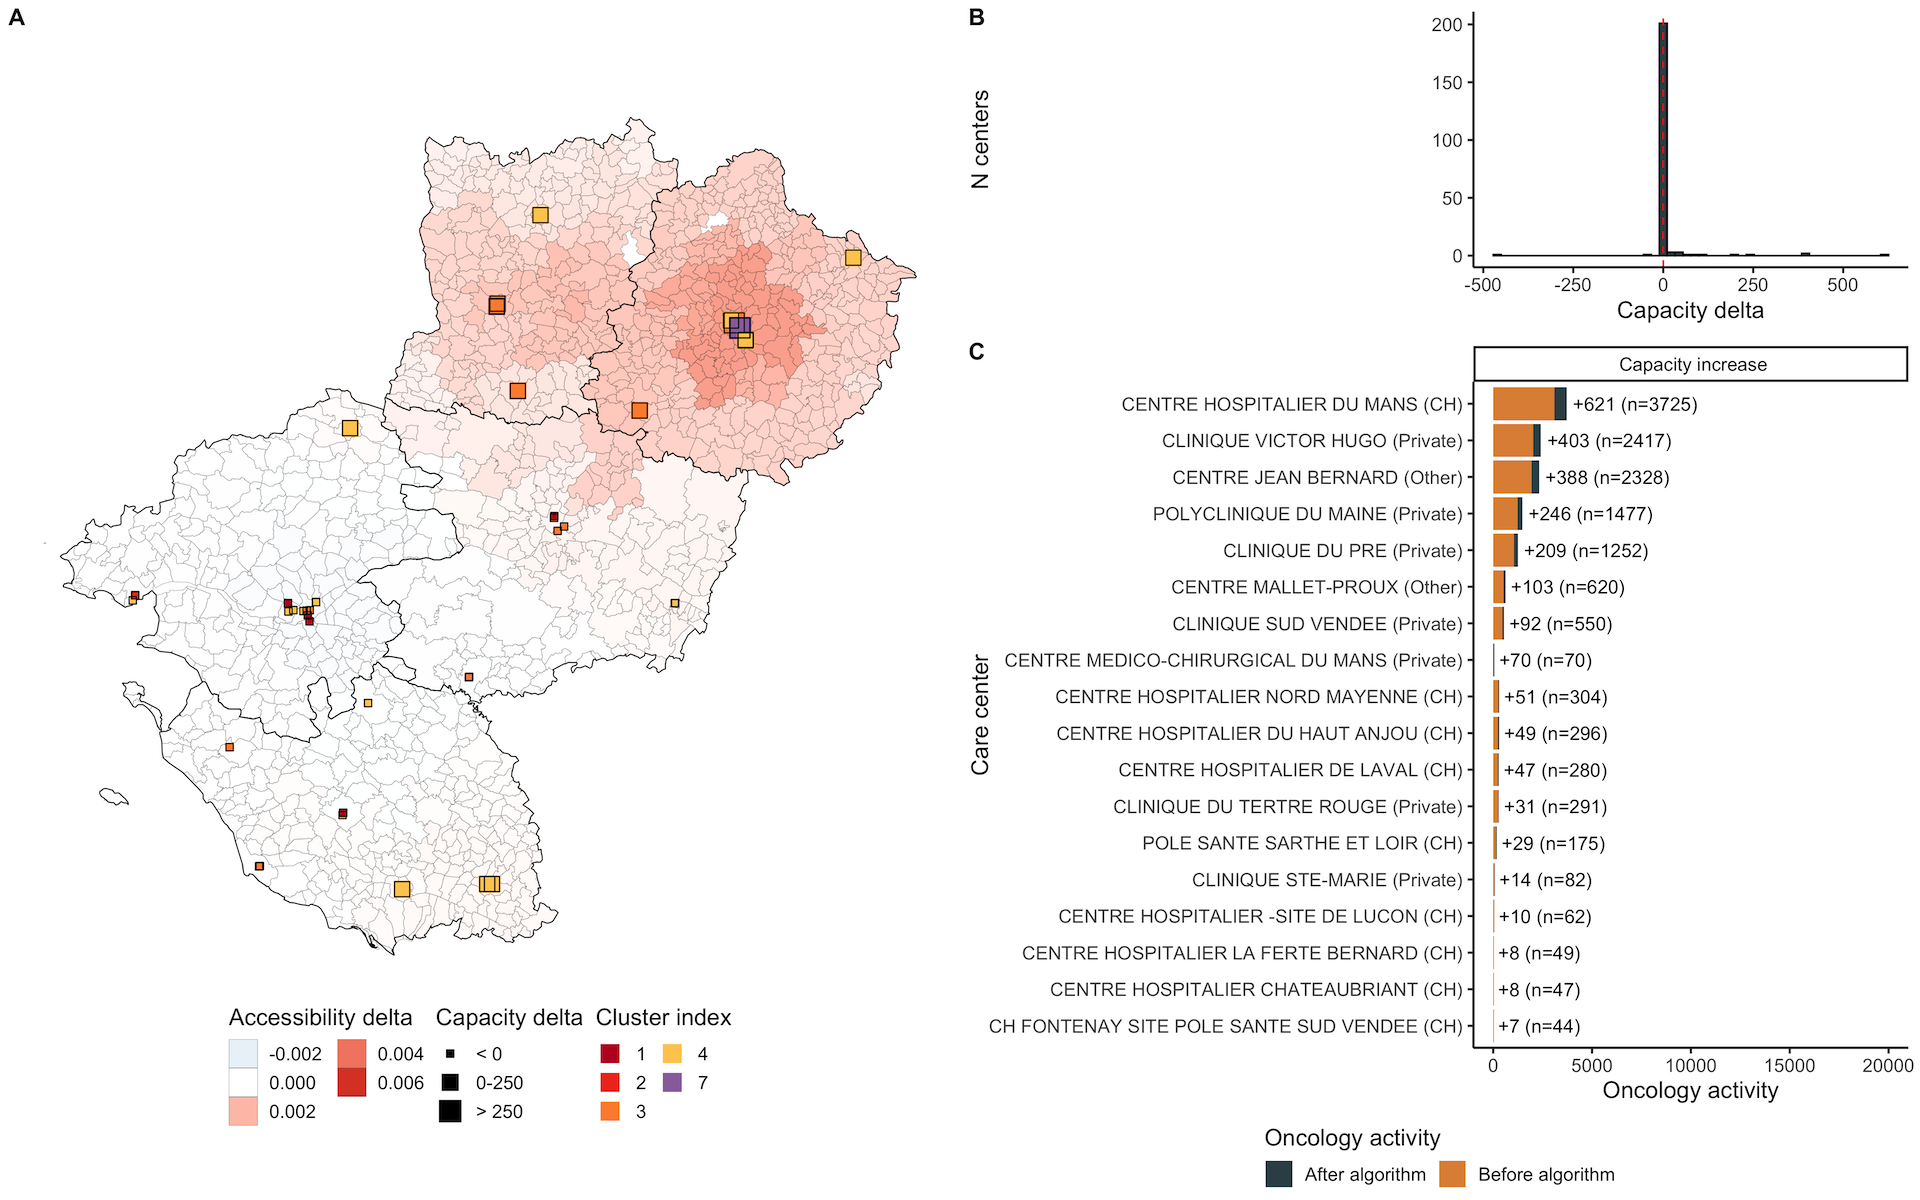
\includegraphics[width=0.9\textwidth]{images/camion/optim_region/optim_Pays-de-la-Loire.png}
    \centering
    \caption{ \textbf{Optimization results in Pays-de-la-Loire.} Additional
        activity was 1,890. 18 centers grew and 2 decreased. Median
        accessibility before optimization was 0.0118 and 0.0121 after,
        corresponding to a 2.4\% increase. Accessibility mainly grew near Le
        Mans, Angers and La Roche sur Yon. }
\end{figure}

\subsection*{Occitanie}

In Occitanie, the additional activity was 3,652. 28 centers grew and 1
decreased. Median accessibility before optimization was 0.0087 and 0.0091 after,
corresponding to a 4.7\% increase. Accessibility mainly grew around Perpignan,
Rodez, Mende and Tarbes. The two largest cities in the region Toulouse and
Montpellier were ignored by the algorithm, since this is where the largest
hospitals already are. The three hospitals that were the most developed by the
algorithm are Clinique Saint Pierre, a private hospital; \ac{ch} Perpignan
which is public and Centre Catalan d'Oncologie Saint Pierre, a private
hospital dedicated to oncology located in Perpignan. The three areas picked
by the algorithm are located apart from each other on the outskirts
of the region.

\begin{figure}[H]
    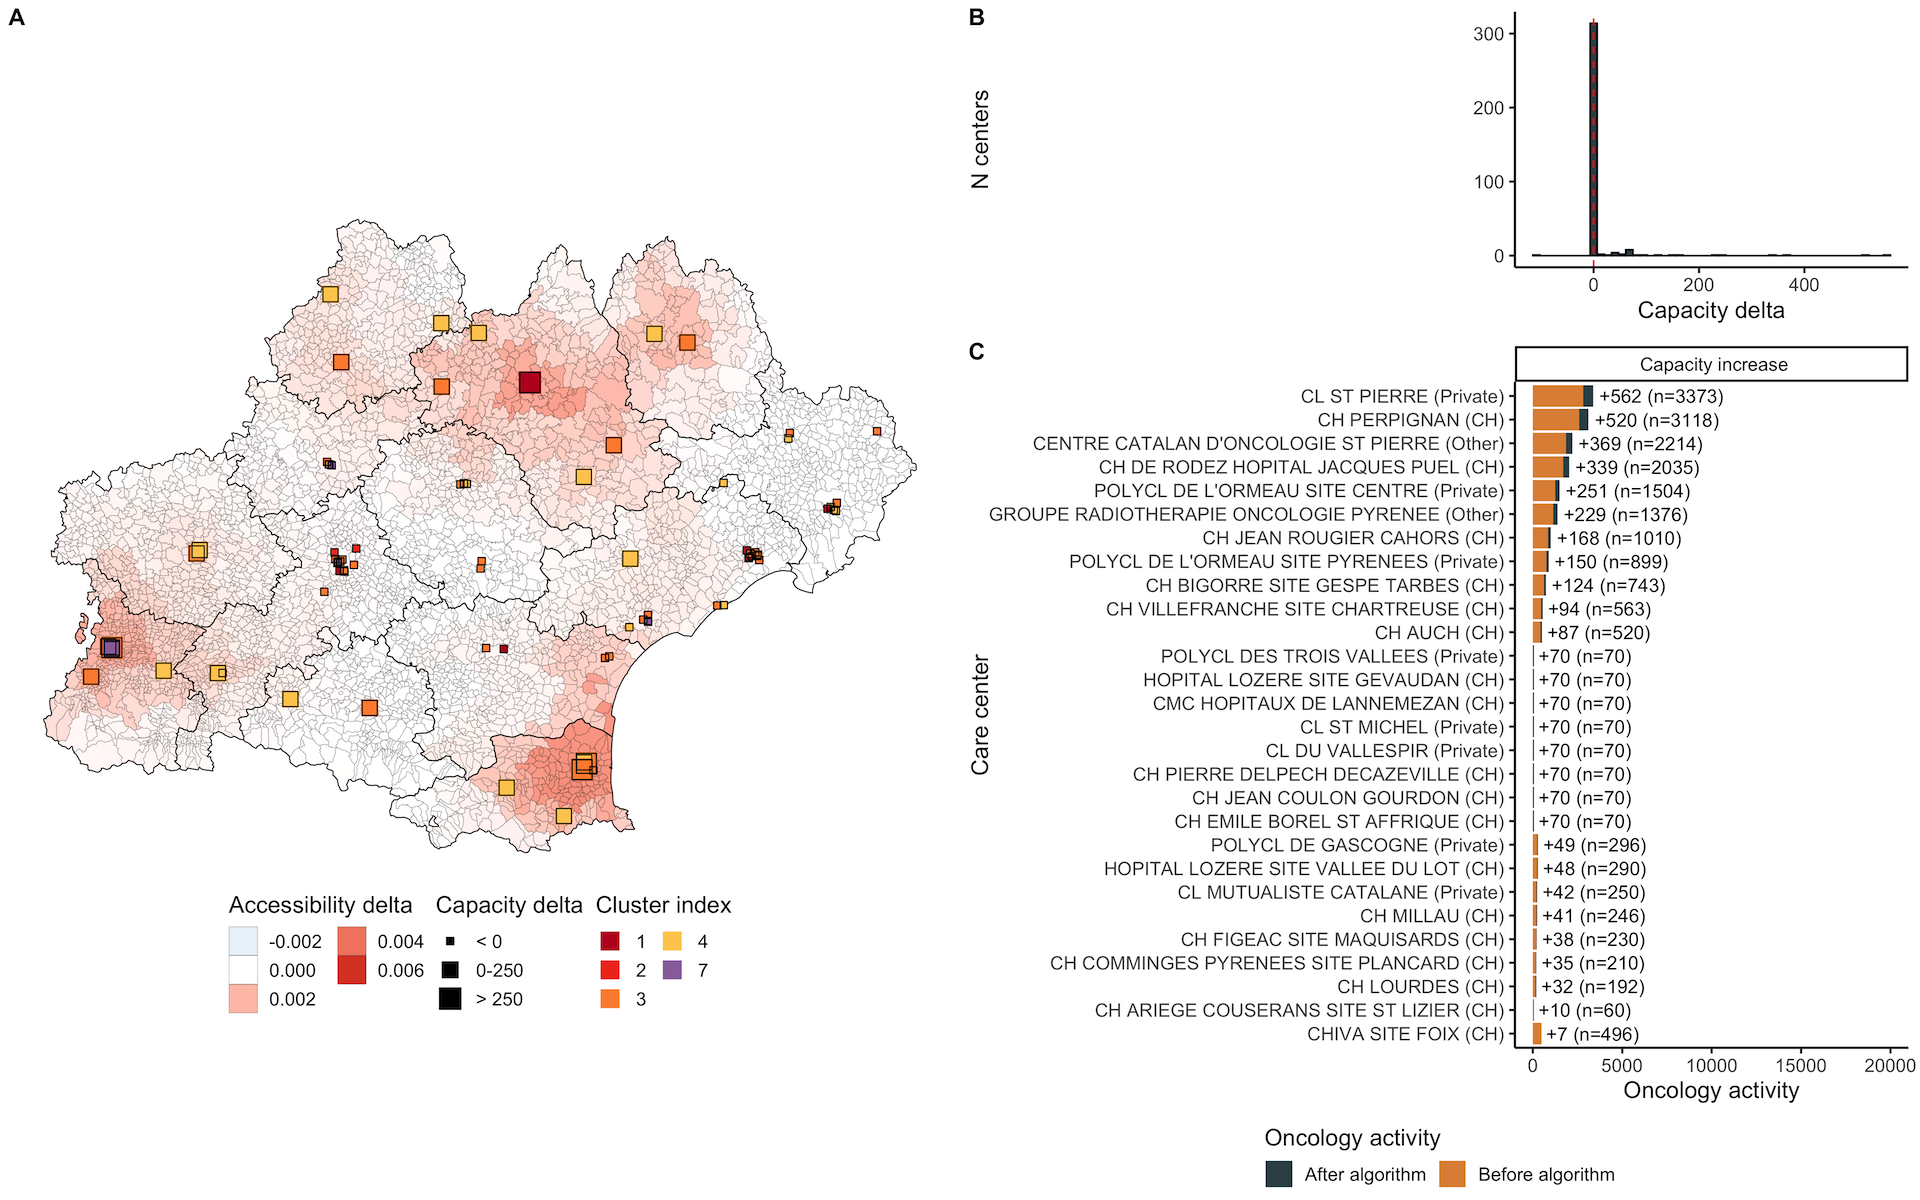
\includegraphics[width=0.9\textwidth]{images/camion/optim_region/optim_Occitanie.png}
    \centering
    \caption{ \textbf{Optimization results in Occitanie.} Additional activity
        was 3,652. 28 centers grew and 1 decreased. Median accessibility before
        optimization was 0.0087 and 0.0091 after, corresponding to a 4.7\%
        increase. Accessibility grew around Perpignan, Rodez, Mende and Tarbes.
    }
\end{figure}

\subsection*{Nouvelle-Aquitaine}

In Nouvelle Aquitaine, the additional activity was 3,445. A total of 25 centers
grew and 1 decreased. The median accessibility before optimization was 0.0117 and
0.0119 after, corresponding to a 1.5\% increase. Accessibility mainly grew around
Limoges, Angoulême, and Brive-la-Gaillarde. Unlike in the Occitanie region,
the algorithm picked areas that are fairly close to each others, mostly located
on the northern east part of the region. The largest city Bordeaux was again
left unchanged by the algorithm. The three hospitals with the largest increase
in capacity are \ac{chru} Dupuytren in Limoges; \ac{ch} Dubois in
Brive-la-Gaillarde and Clinique François Chenieux in Limoges.

\begin{figure}[H]
    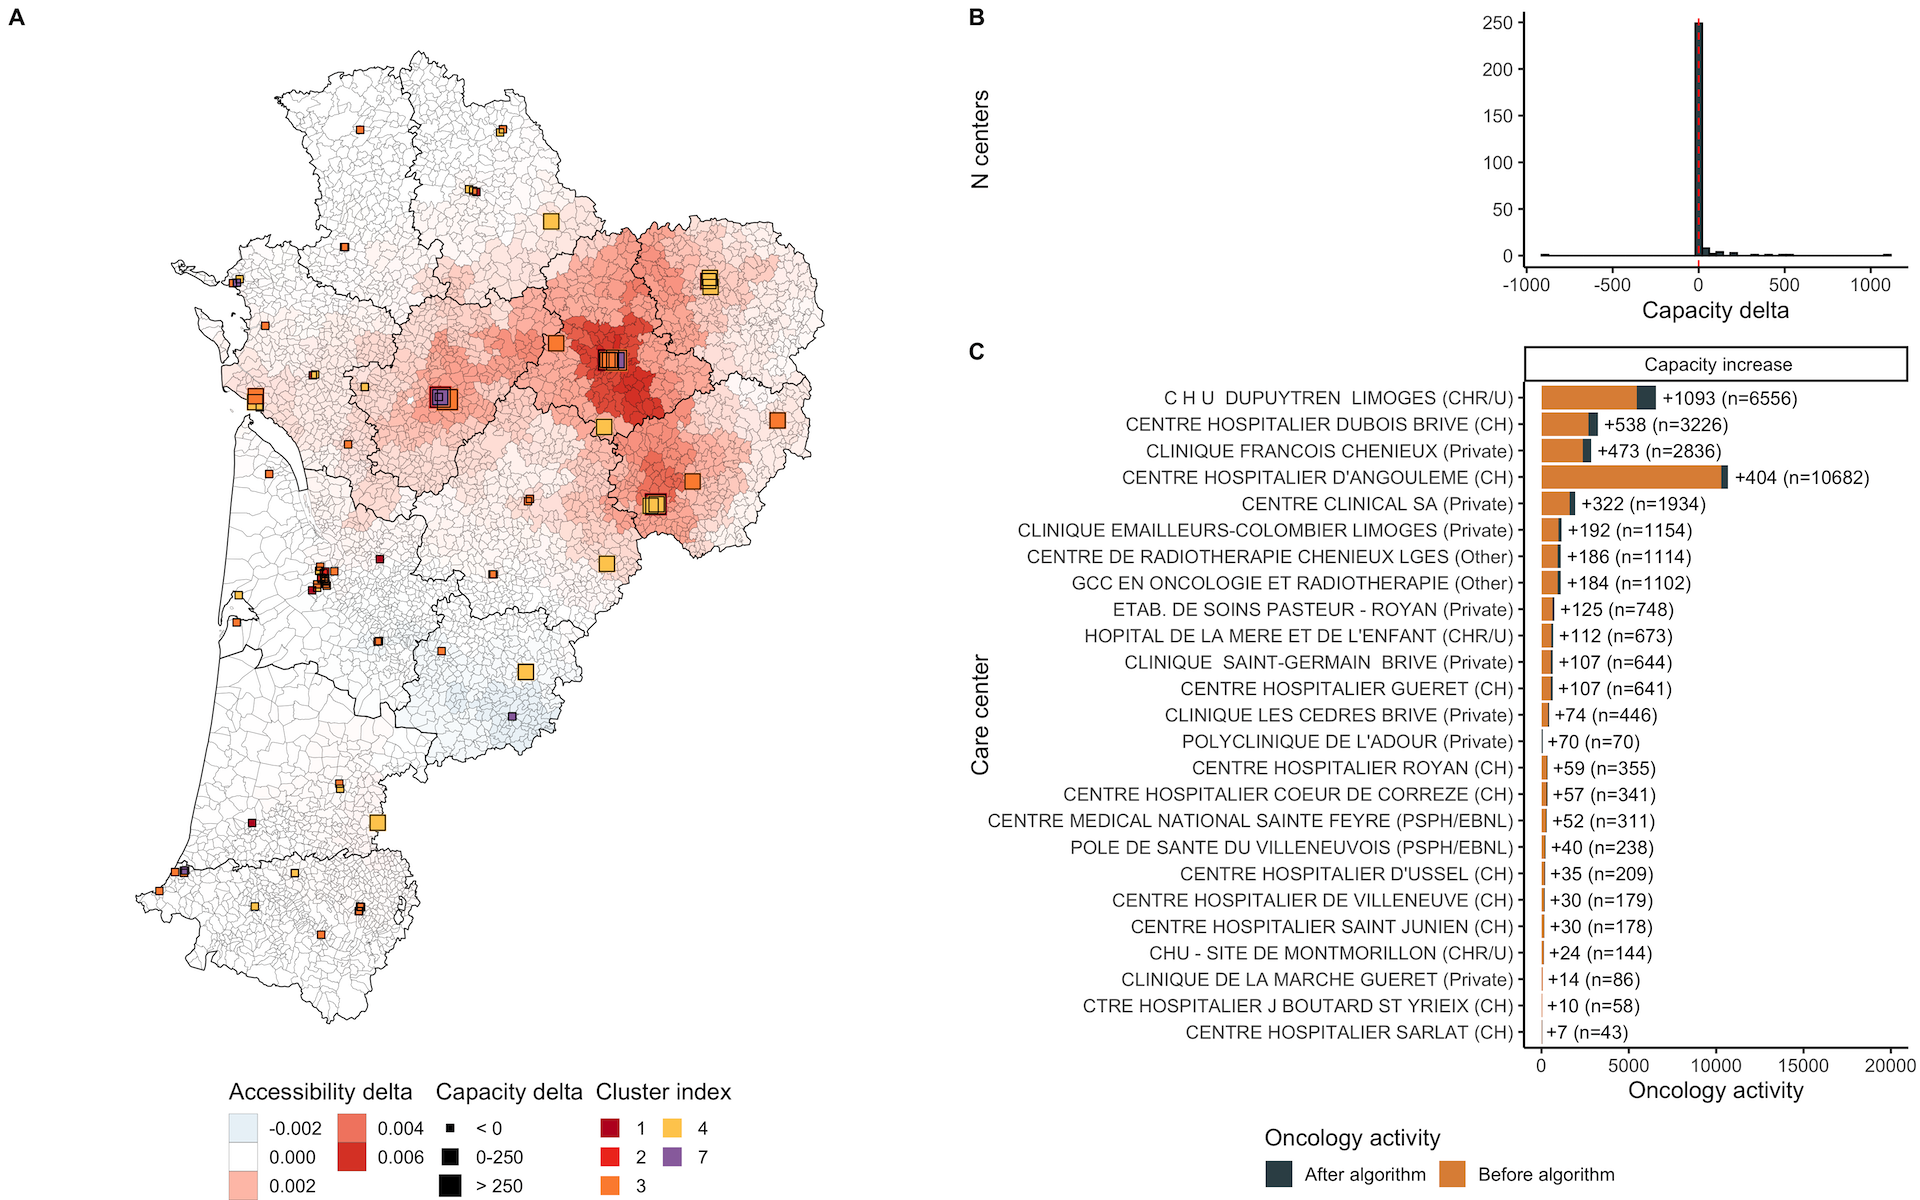
\includegraphics[width=0.9\textwidth]{images/camion/optim_region/optim_Nouvelle-Aquitaine.png}
    \centering
    \caption{ \textbf{Optimization results in Nouvelle-Aquitaine.} Additional
        activity was 3,445. 25 centers grew and 1 decreased. Median
        accessibility before optimization was 0.0117 and 0.0119 after,
        corresponding to a 1.5\% increase. Accessibility grew around Limoges,
        Angouleme, and Brive-la-Gaillarde. }
\end{figure}

\subsection*{Normandie}

In Normandie, the additional activity was 1,523. A total of 15 centers grew and
none decreased. The median accessibility before optimization was 0.0105 and 0.0106 after,
corresponding to a 1\% increase. Accessibility mostly grew near Caen, Argentan, and
St-Lo, on the middle-western part of the region. Hospitals near Rouen and Évreux
were left unchanged by the optimization process. The algorithm mostly targeted
a single hospital: the \ac{chru} Cote de Nacre, a public university hospital in
Caen. This hospital received a +771 activity, for a total of 4628 stays. The
other hospitals that were increased are smaller, and their number of stays
range between 24 and 725.

\begin{figure}[H]
    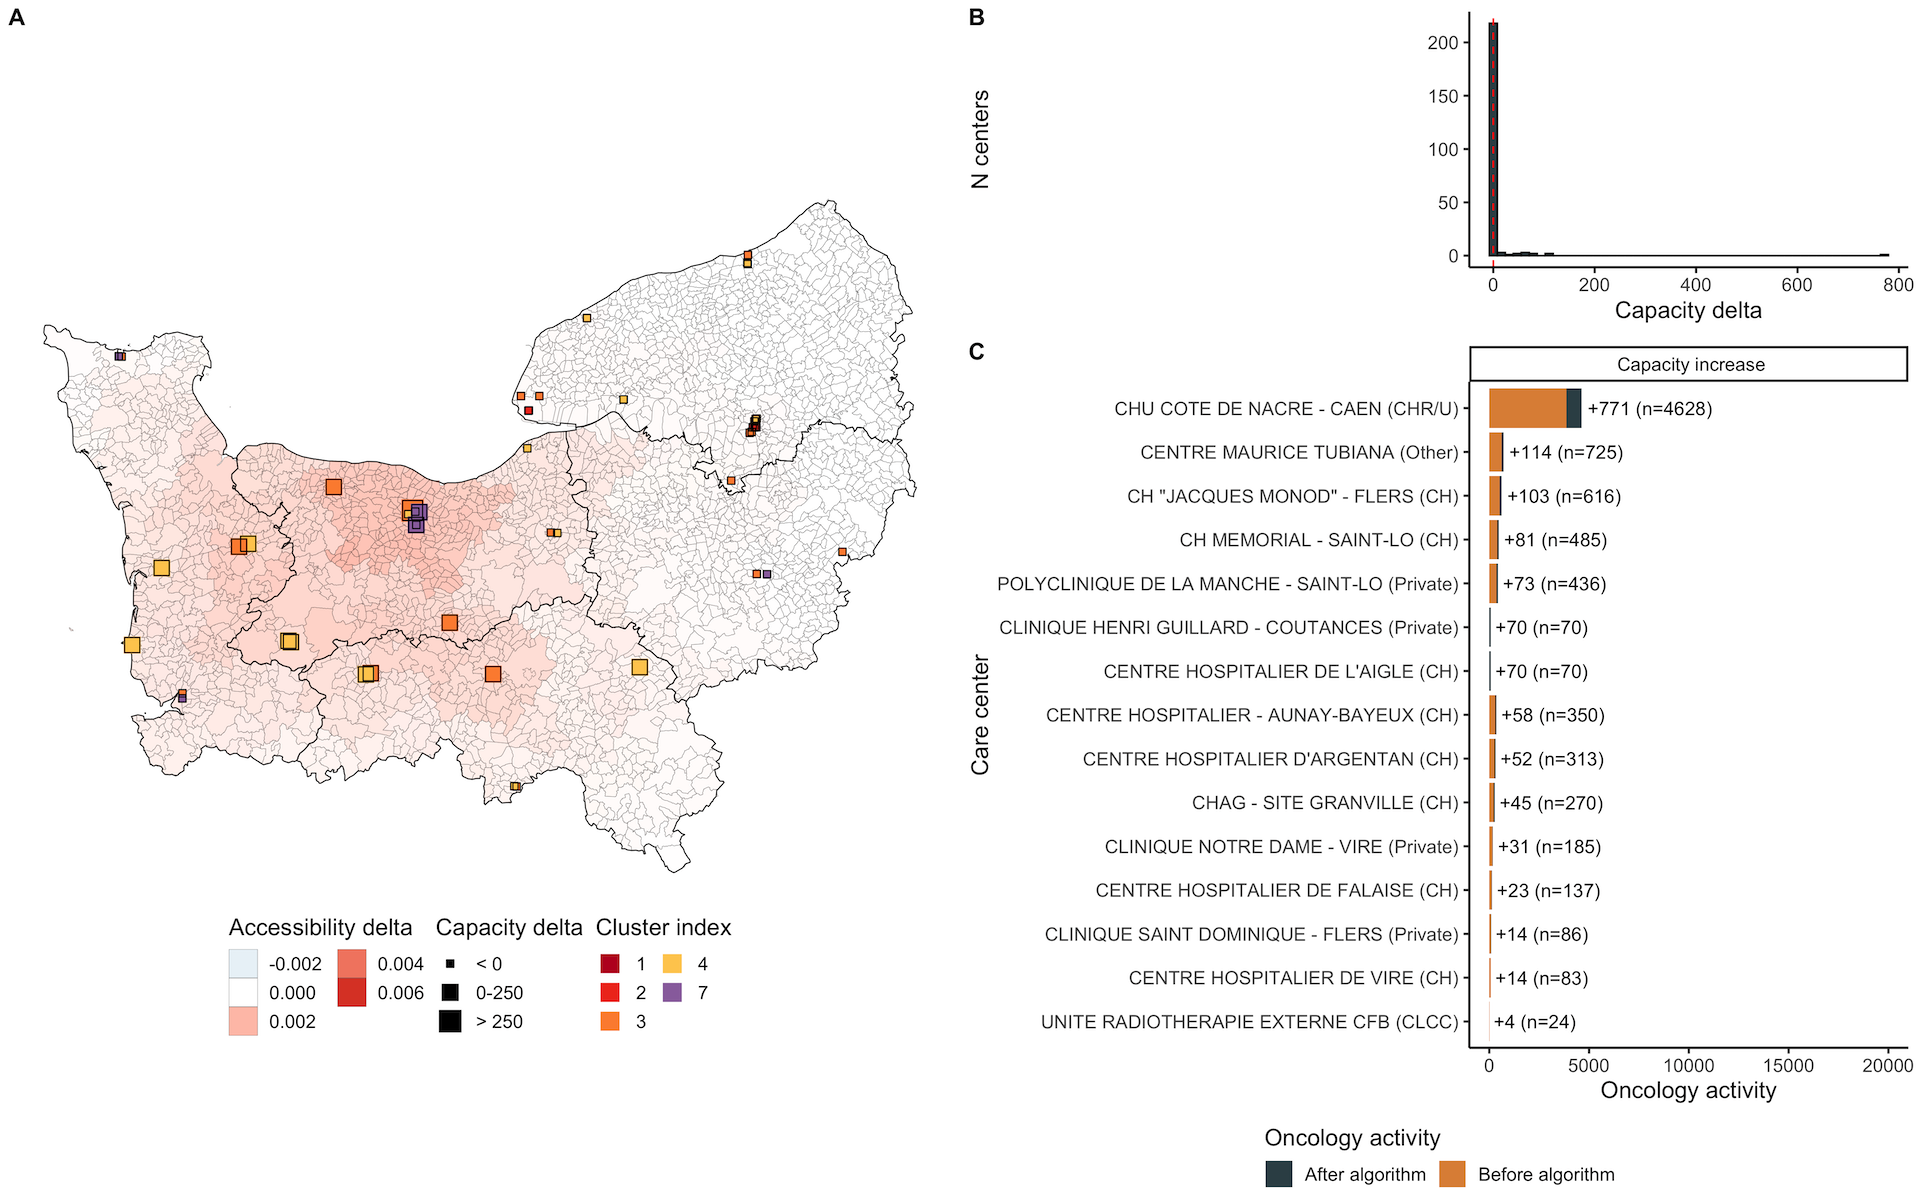
\includegraphics[width=0.9\textwidth]{images/camion/optim_region/optim_Normandie.png}
    \centering
    \caption{ \textbf{Optimization results in Normandie.} Additional activity
        was 1,523. 15 centers grew and 0 decreased. Median accessibility before
        optimization was 0.0105 and 0.0106 after, corresponding to a 1\%
        increase. Accessibility grew near Caen, Argentan, and St-Lo. }
\end{figure}

\subsection*{Île-de-France}

In Ile-de-France, the additional activity was 5,826. 44 centers grew and 1
decreased. The median accessibility before optimization was 0.0088 and
0.0089 after, corresponding to a 1.3\% increase. Accessibility grew
around Mantes-la-Jolie, Rambouillet, Melun, and Évry, on the outskirt of the
region, surrounding the Paris city. Looking at the map, it is harder to
distinguish specific areas that were developed, since the accessibility
increase is much more spread than in the other regions. This is probably
due to the relatively high population densities in the whole region. Developing
the hospitals outside of the Paris city seems fair, given the tedious drive
that it would take to reach the city center from the suburbs, especially due to
the traffic. Moreover, the most specialized hospitals in Paris are often
already saturated, from patients living in Paris or coming from other regions
in the case of rare cancers.

\begin{figure}[H]
    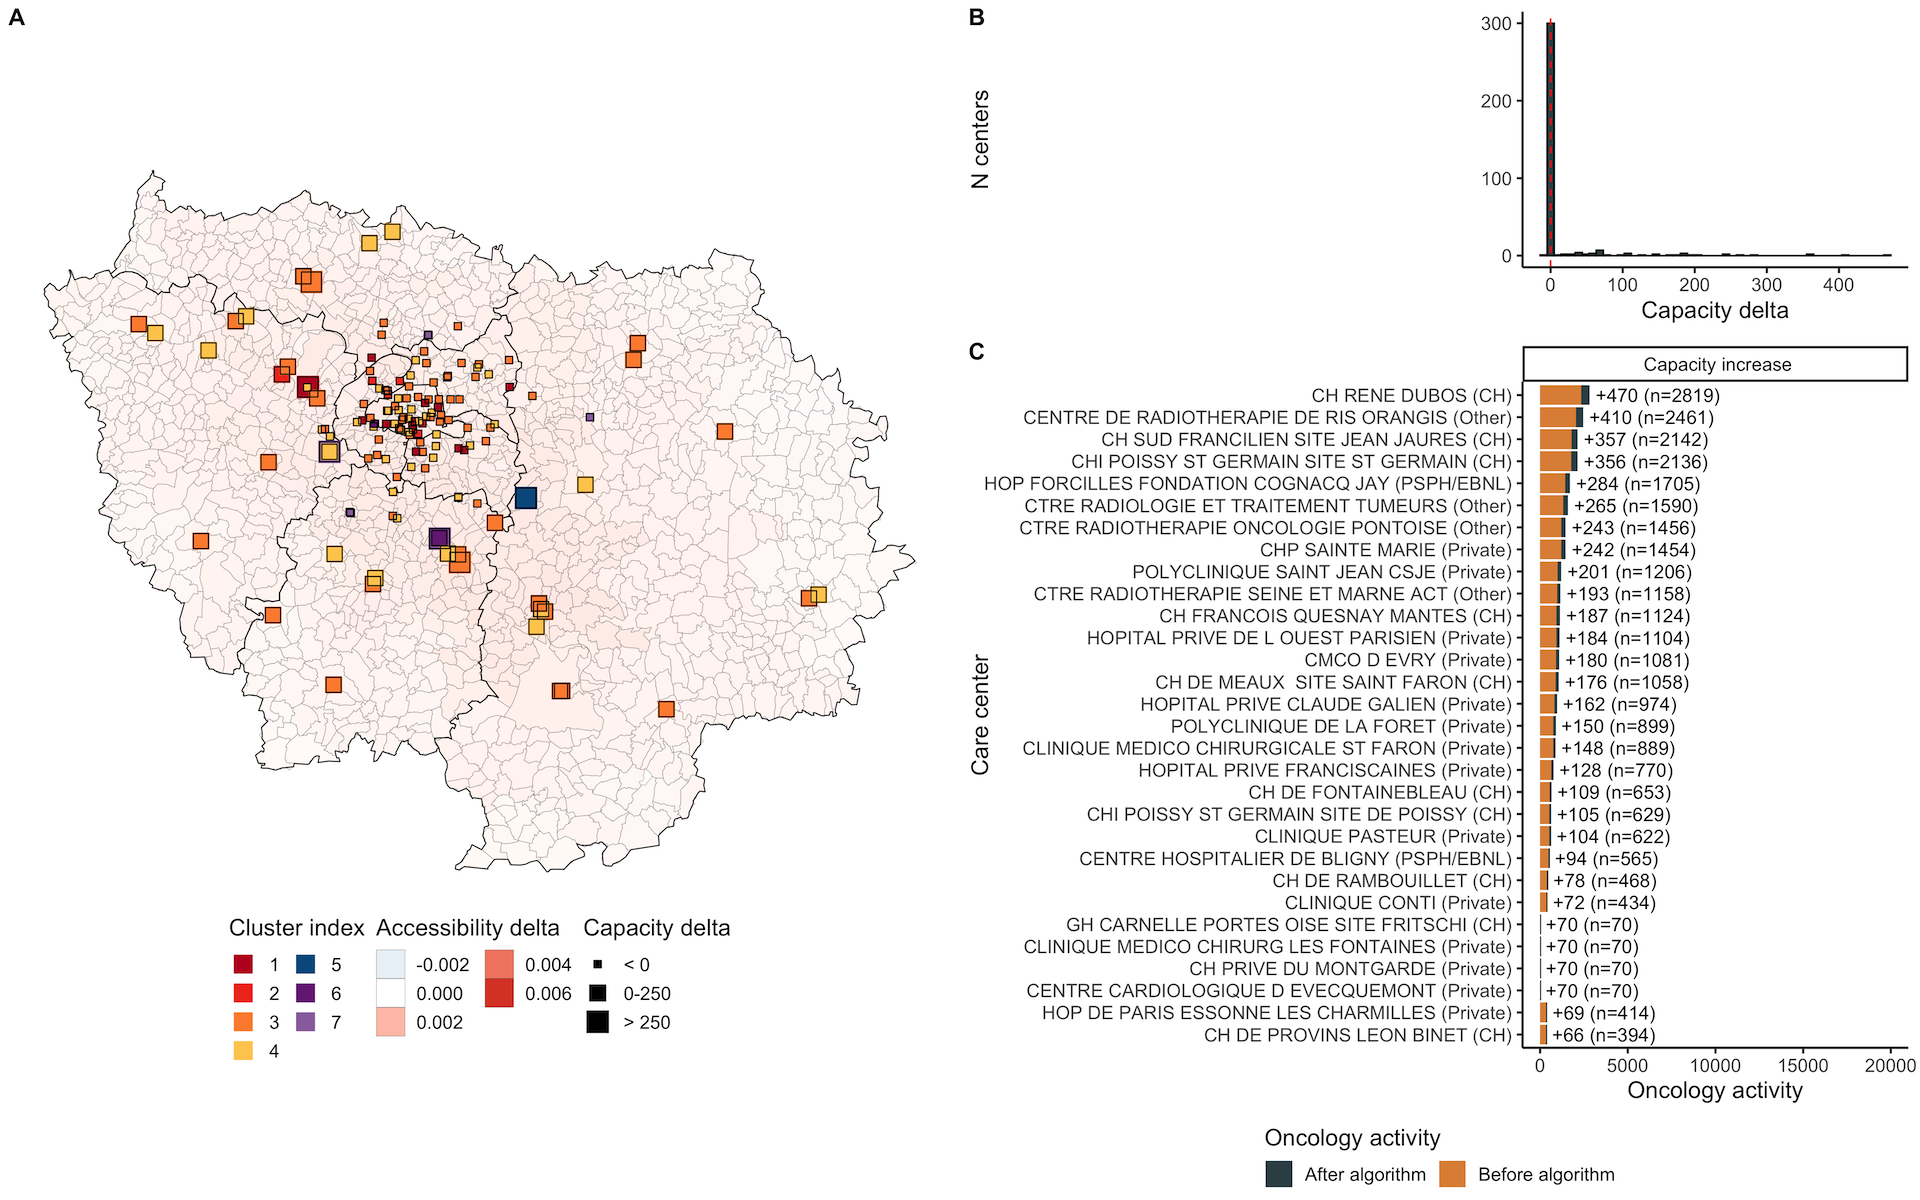
\includegraphics[width=0.9\textwidth]{images/camion/optim_region/optim_Ile-de-France.png}
    \centering
    \caption{ \textbf{Optimization results in Ile-de-France.} Additional
        activity was 5,826. 44 centers grew and 1 decreased. Median
        accessibility before optimization was 0.0088 and 0.0089 after,
        corresponding to a 1.3\% increase. Accessibility grew around
        Mantes-la-Jolie, Rambouillet, Melun, and Évry. }
\end{figure}

\subsection*{Hauts-de-France}

In Hauts-de-France, the additional activity was 2,520. A total of 29 centers
grew and 1 decreased. The median accessibility before optimization was 0.01 and
0.0102 after, corresponding to a 2.1\% increase. Accessibility mainly grew
around St-Quentin and Valenciennes. Similarly to the results in Ile-de-France
region, it is relatively hard to distinguish precise areas where the accessibility
was increased, and the accessibility delta is more evenly spread around the region.
However there are areas where the hospitals remained unchanged, in Lille for instance or
in the southern part of the region, in the Oise department, near Beauvais,
Compiègne or Senlis. The two hospitals where the capacity increase were the
largest are Centre Leonard de Vinci, a private structure near Douai; \ac{ch}
Saint Quentin, a public hospital. Both received around +500 capacity increase,
bringing them to a total of roughly 3000.

\begin{figure}[H]
    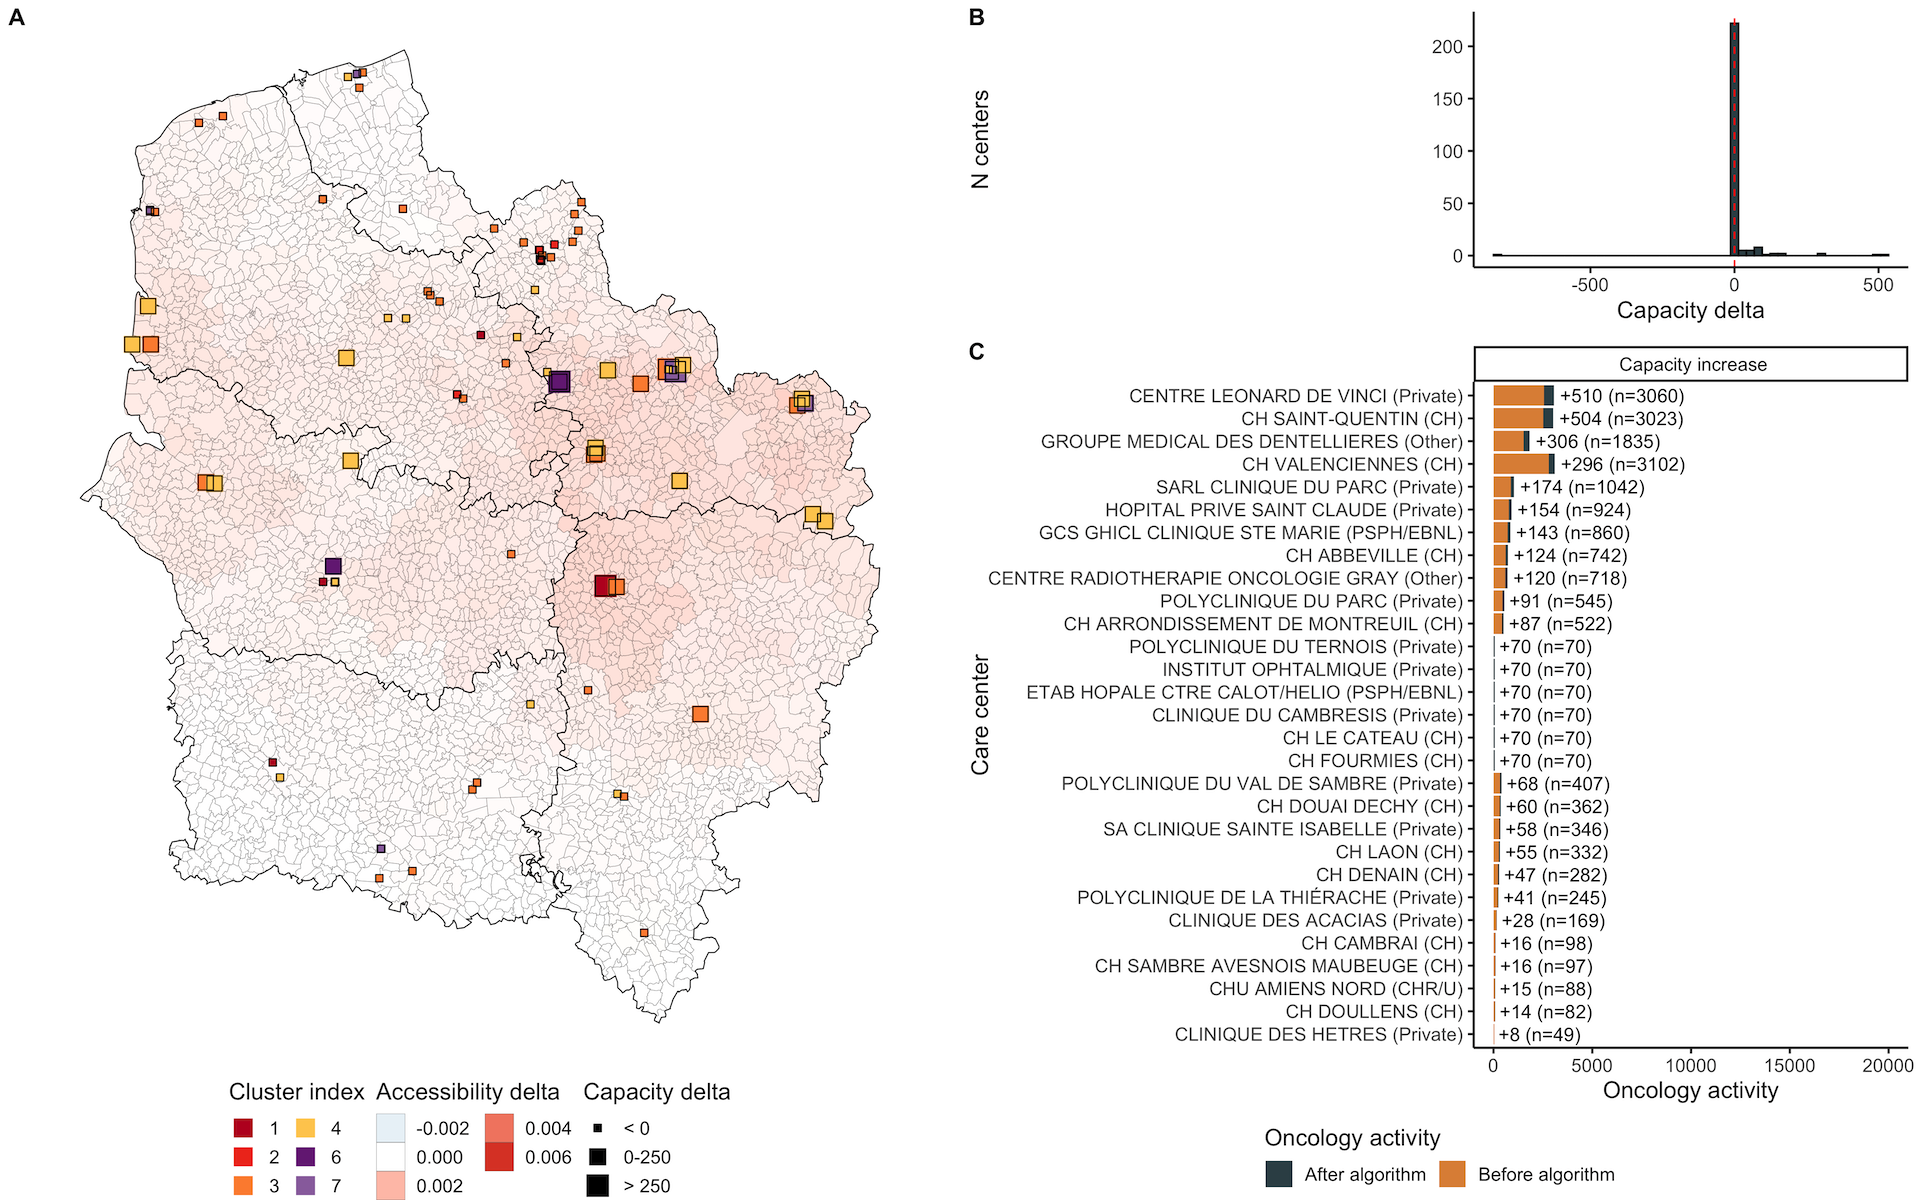
\includegraphics[width=0.9\textwidth]{images/camion/optim_region/optim_Hauts-de-France.png}
    \centering
    \caption{ \textbf{Optimization results in Hauts-de-France.} Additional
        activity was 2,520. 29 centers grew and 1 decreased. Median
        accessibility before optimization was 0.01 and 0.0102 after,
        corresponding to a 2.1\% increase. Accessibility grew around St-Quentin
        and Valenciennes. }
\end{figure}

\subsection*{Grand Est}

In Grand Est, the Additional activity was 2,663. A total of 31 centers grew and 4
decreased. The median accessibility before optimization was 0.0096 and
0.0099 after, corresponding to a 3\% increase. Accessibility grew around
Troyes and Épinal. In this region, the municipalities with the largest accessibility
scores are located on the eastern end, along the Germany frontier. The hospitals
in these areas were not increased, and the algorithm focused on sub-urban
cities like Troyes, where patients are sometimes traveling all the way to Paris
for certain types of cancer. Among the grown hospitals, the first two ones are
in Troyes. Clinique de Champagne, a private structure, received an additional
activity of 543, totalling 3260 stays. Next, the \ac{ch} Troyes, a public hospital
received 375 additional stays, bringing the capacity to 2248.

\begin{figure}[H]
    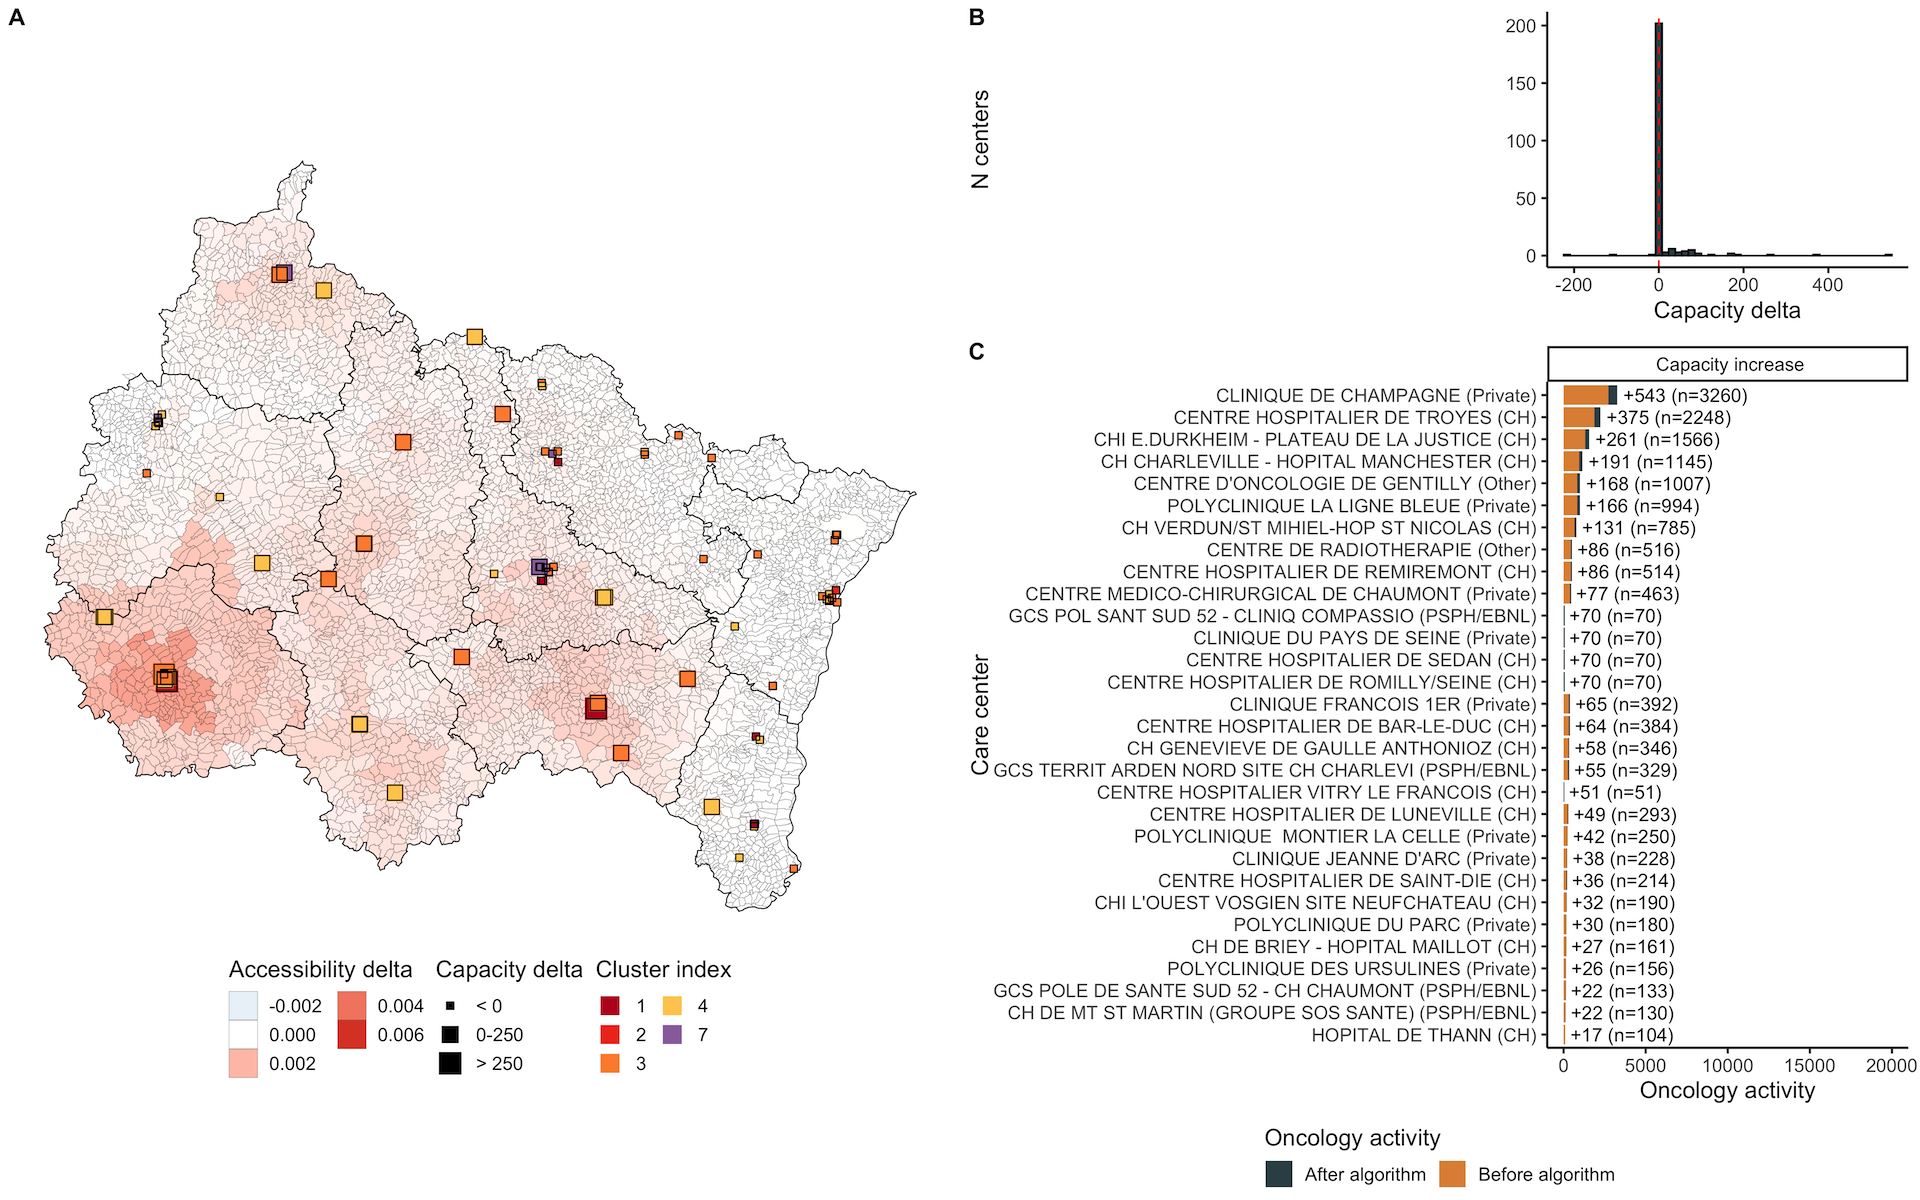
\includegraphics[width=0.9\textwidth]{images/camion/optim_region/optim_Grand-Est.png}
    \centering
    \caption{ \textbf{Optimization results in Grand-Est.} Additional activity
        was 2,663. 31 centers grew and 4 decreased. Median accessibility before
        optimization was 0.0096 and 0.0099 after, corresponding to a 3\%
        increase. Accessibility grew around Troyes and Épinal. }
\end{figure}

\subsection*{Centre-Val de Loire}

In Centre-Val de Loire, the additional activity was 1,072. A total of 10 centers
grew and 1 decreased. The median accessibility before optimization was 0.0099 and
0.0102 after, corresponding to a 2.9\% increase. Accessibility grew around
Bourges and Châteauroux areas. Compared to the other regions, very few hospitals
were increased by the algorithm. Two departments were affected by the modifications:
Indre and Cher. Cities like Tours, Chartres and Orleans were left as such by
the optimization process. The two hospitals that were the most affected by the
algorithm are private structures, that each received around 200 capacity increase.

\begin{figure}[H]
    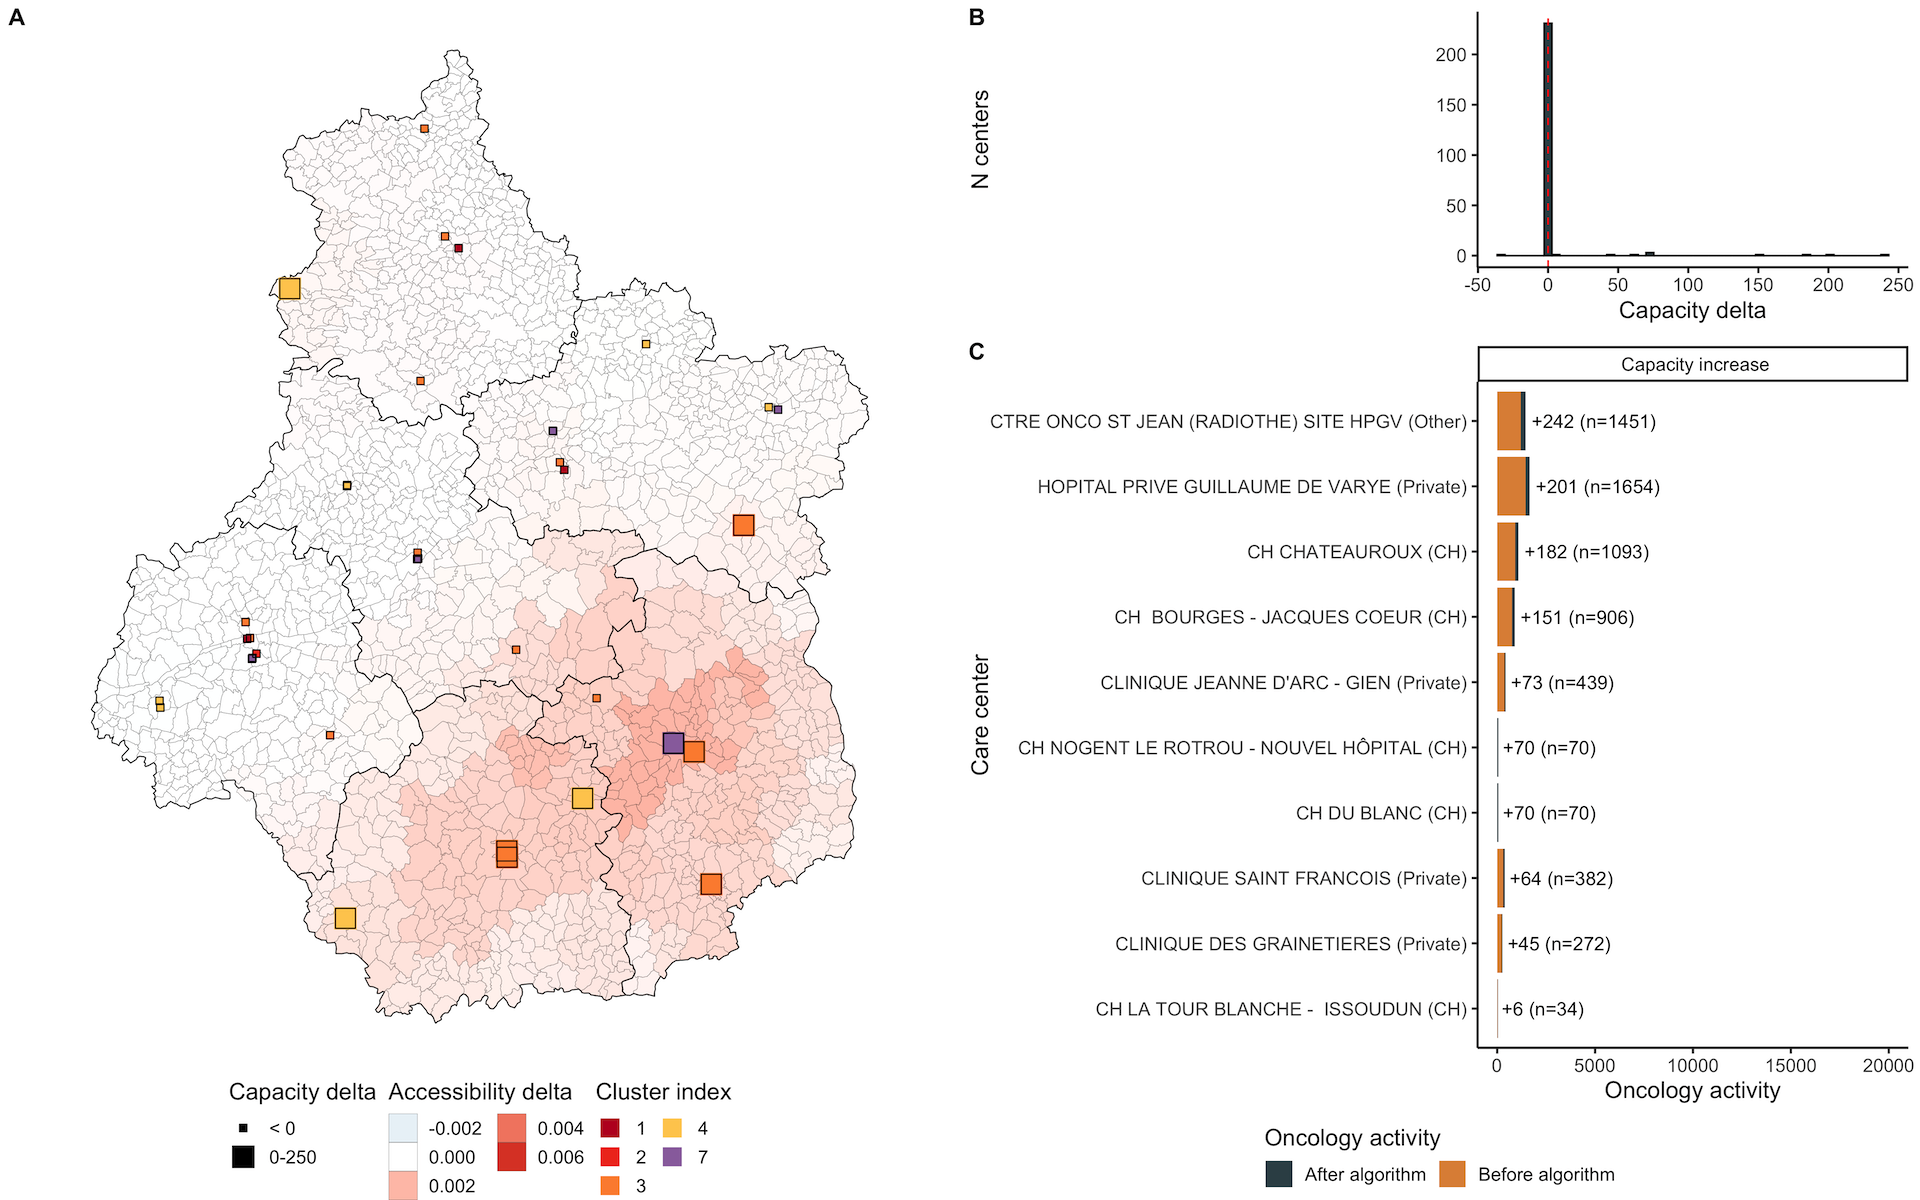
\includegraphics[width=0.9\textwidth]{images/camion/optim_region/optim_Centre-Val-de-Loire.png}
    \centering
    \caption{ \textbf{Optimization results in Centre-Val-de-Loire.} Additional
        activity was 1,072. 10 centers grew and 1 decreased. Median
        accessibility before optimization was 0.0099 and 0.0102 after,
        corresponding to a 2.9\% increase. Accessibility grew around
        Bourges and Châteauroux. }
\end{figure}

\subsection*{Bretagne}

In Bretagne, the additional activity was 1,773. A total of 10 centers grew and
2 decreased. The median accessibility before optimization was 0.0131 and 0.0134 after,
corresponding to a 2.4\% increase. The accessibility grew mostly around St-Brieuc area,
in the northern part of the region. The accessibility distribution in Bretagne
was among the highest and most homogeneous compared to the other regions.
Accessibility was lower in the inland areas between Cotes d'Armor and Morbihan
departments. This optimization affected mostly the Cotes d'Armor department, but
spread near the frontier of Morbihan. Since the population density is lower in
the center part of the region, the algorithm focused on the hospitals located
in the sub-urban areas near Saint Brieuc. We pointed earlier that even though
the accessibility in the inland part of the region was not as high as on the
outskirts, the patients average travel duration remained relatively low,
limiting the travel burden.

\begin{figure}[H]
    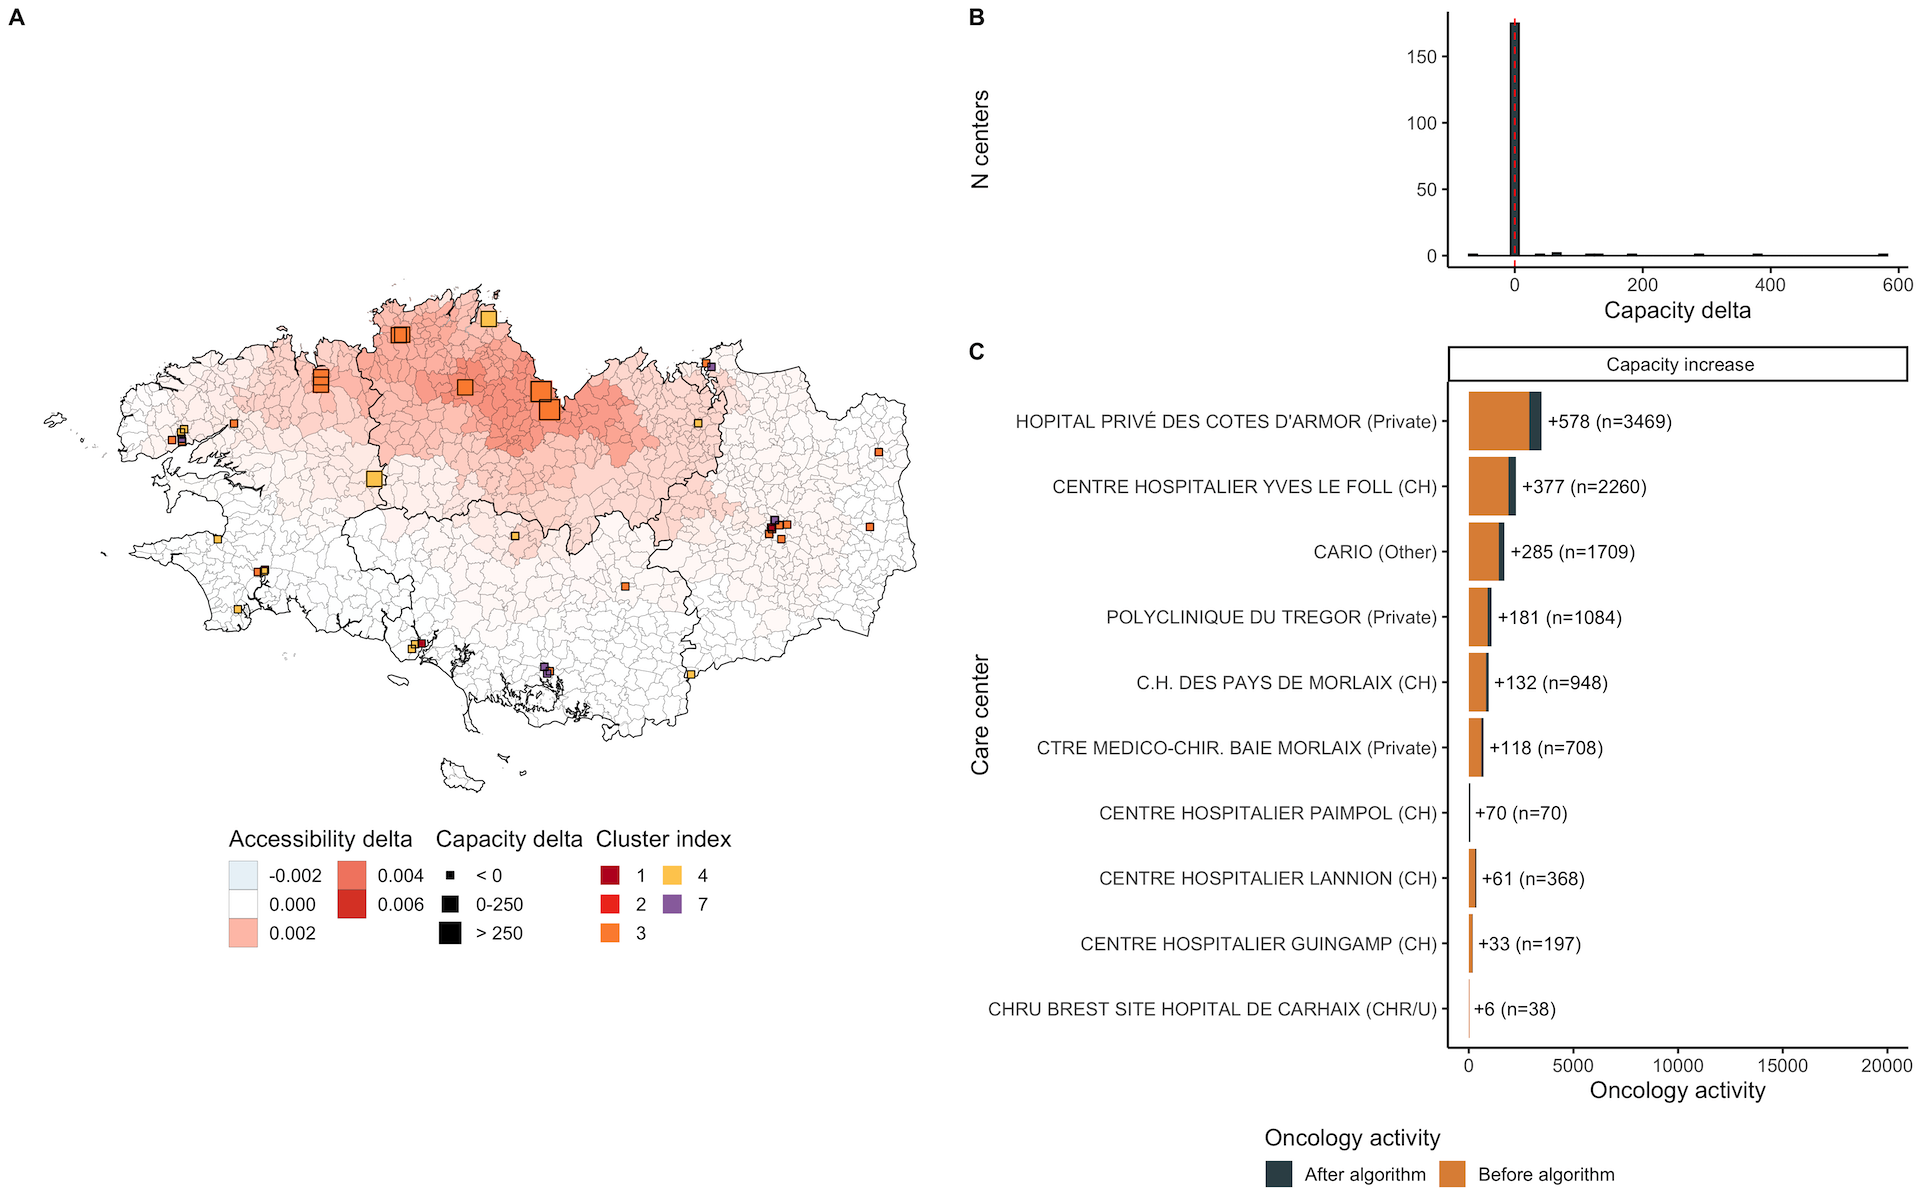
\includegraphics[width=0.9\textwidth]{images/camion/optim_region/optim_Bretagne.png}
    \centering
    \caption{ \textbf{Optimization results in Bretagne.} Additional activity was
        1,773. 10 centers grew and 2 decreased. Median accessibility before
        optimization was 0.0131 and 0.0134 after, corresponding to a 2.4\%
        increase. Accessibility grew around St-Brieuc. }
\end{figure}

\subsection*{Bourgogne-Franche-Comté}

In Bourgogne-Franche-Comté, the Additional activity was 1,330. A total of 13
centers grew while none decreased. The Median accessibility before optimization
was 0.0096 and 0.0098 after, corresponding to a 1.9\% increase. Accessibility grew
around Nevers and Auxerre, on the western side of the region. The largest hospitals
in this region are located near Dijon, the largest city. The hospitals in this
area were left unchanged. The optimization had the largest effect on departments
like Nièvre and Yonne. The number of modified hospitals is relatively low compared
to the other regions, and the largest additional capacities are in the hundreds.
Among the most affected hospitals, two of them are located in Auxerre: the
\ac{ch} Auxerre which is a public structure; and the Centre de Radiothérapie
du Parc, dedicated to radiotherapy.

\begin{figure}[H]
    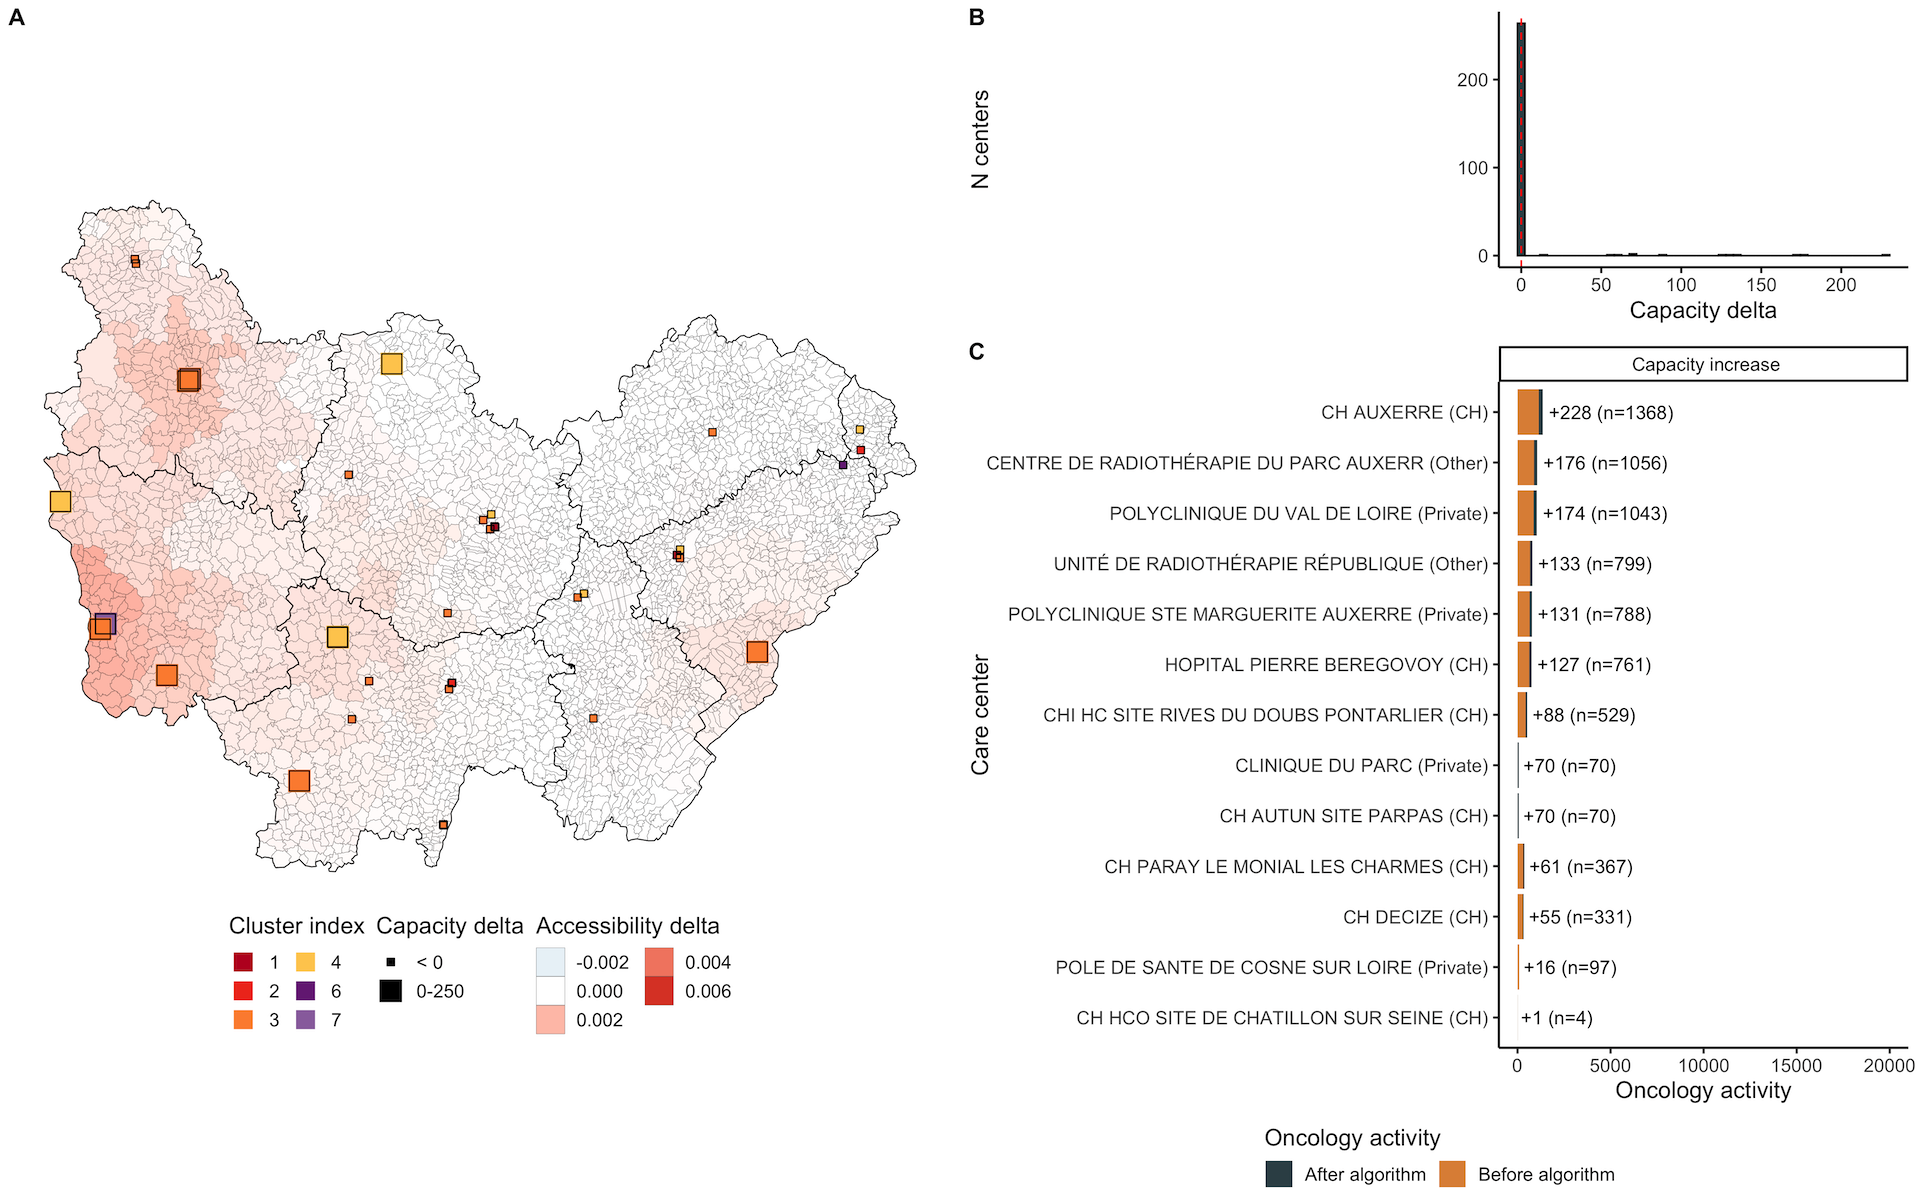
\includegraphics[width=0.9\textwidth]{images/camion/optim_region/optim_Bourgogne-Franche-Comte.png}
    \centering
    \caption{ \textbf{Optimization results in Bourgogne-Franche-Comté.}
        Additional activity was 1,330. 13 centers grew and 0 decreased. Median
        accessibility before optimization was 0.0096 and 0.0098 after,
        corresponding to a 1.9\% increase. Accessibility grew around Nevers,
        Belfort, Vesoul and Auxerre. }
\end{figure}

\subsection*{Auvergne-Rhône-Alpes}

In Auvergne-Rhône-Alpes, the additional activity was 3,883. A total of 23
centers grew and 2 decreased. The median accessibility before optimization was
0.0092 and 0.0095 after, corresponding to a 3.2\% increase. Accessibility grew
around Moulins, Montluçon, Le Puy en Velay, Clermont-Ferrand and Aurillac. The
departments that were the most affected by the capacity increase were Allier,
Puy de Dome, Cantal and Haute Loire, mainly on the eastern part of the region.
The hospitals near Lyon in Rhone department were left unchanged. Developing
the hospitals in the eastern part makes sense to avoid patients traveling from
there to Lyon. Indeed, the routes can be tedious, and the drives relatively
long. The hospital that was developed the most is \ac{clcc} Jean Perrin in
Clermont-Ferrand, a large oncology dedicated hospital. The algorithm allocated
an additional capacity of 1,171, bringing the hospital to a 7,024 overall
activity. In this region, we notice that multiple hospitals from the cluster 1
were developed. In other regions, such hospitals are most of the time ignored
by the algorithm, and structures from cluster 3 or 4 are often developed instead.
Developing hospitals from cluster 1 might be easier than developing hospitals
from least specialized clusters because they have more oncology services that
are already established. However, we must make sure they are not already
saturated, due to the higher oncology volumes they usually operate at.

\begin{figure}[H]
    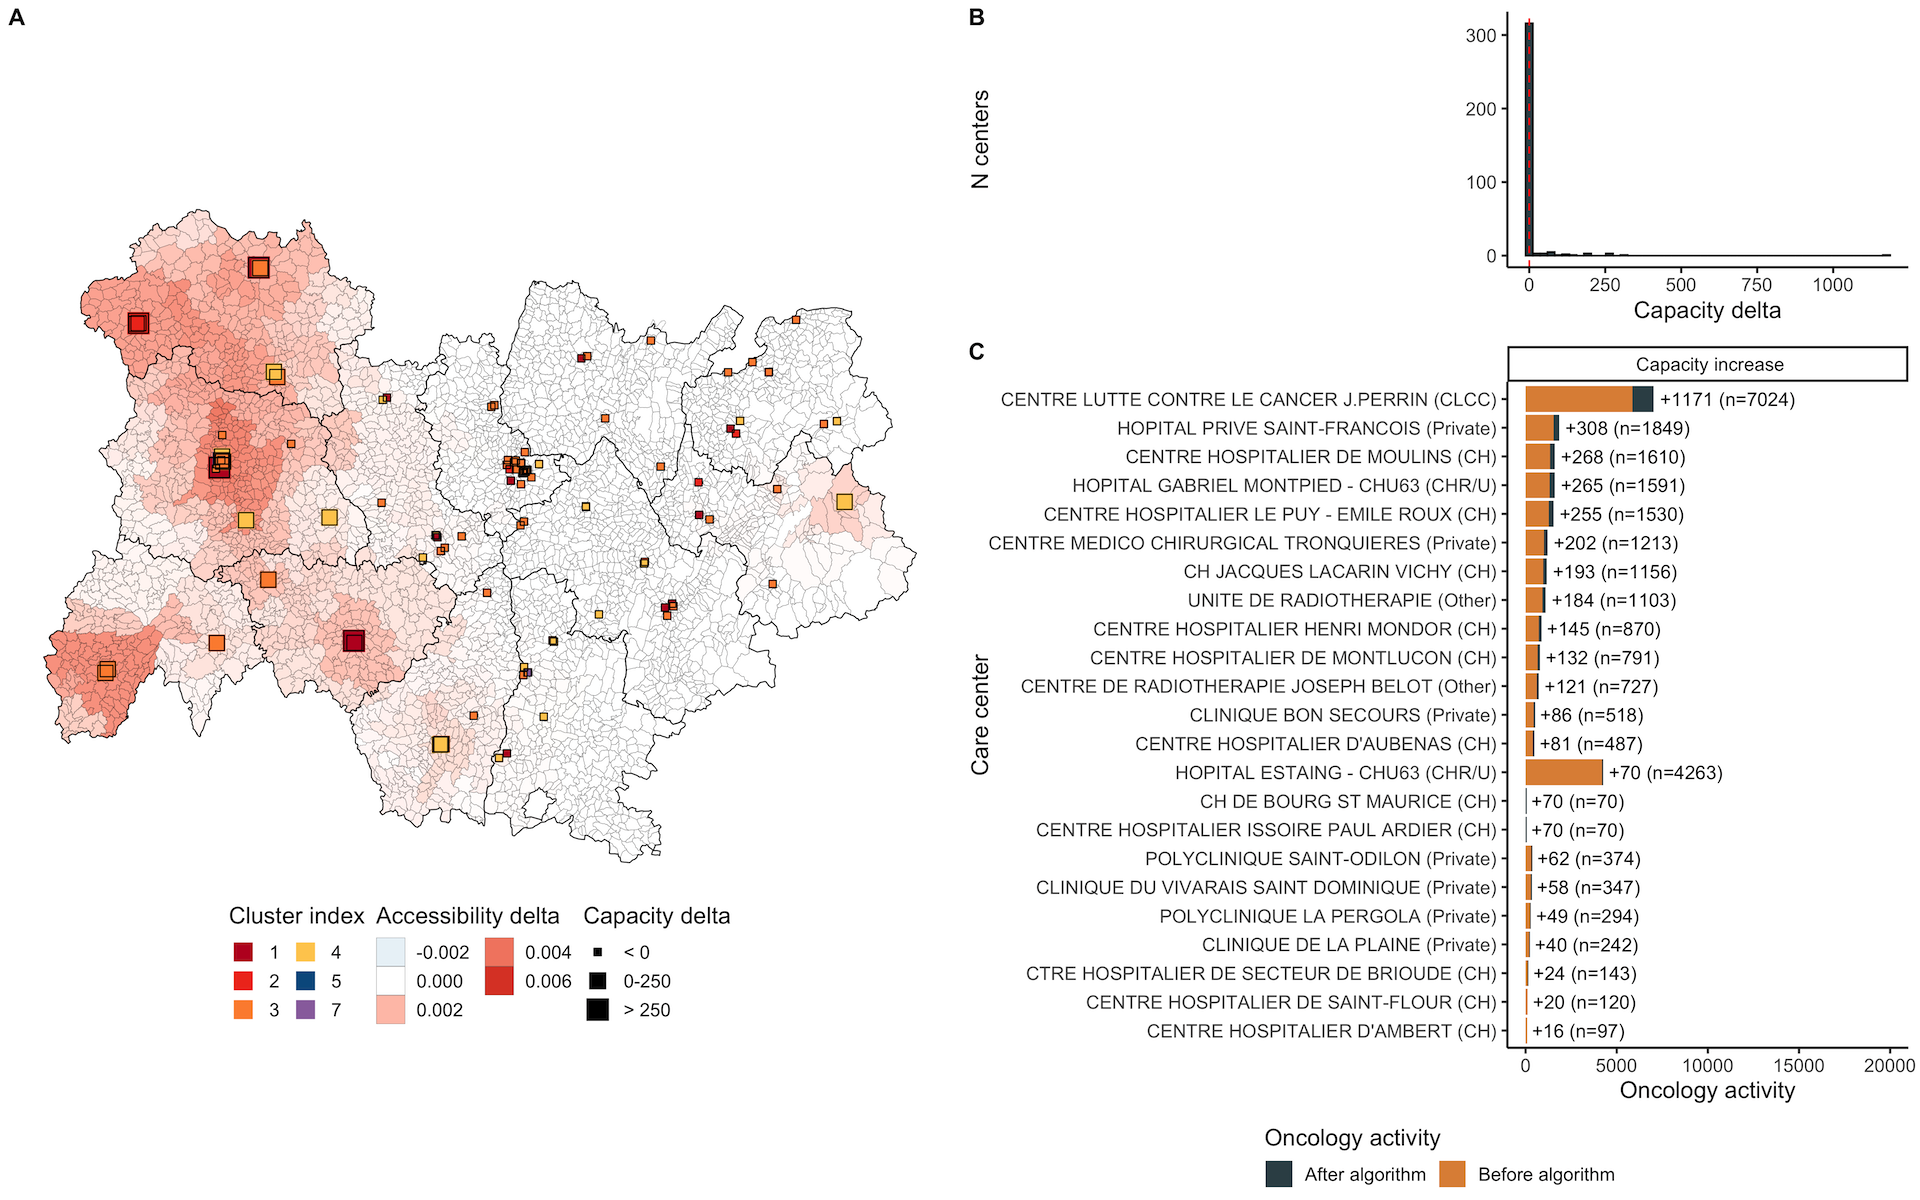
\includegraphics[width=0.9\textwidth]{images/camion/optim_region/optim_Auvergne-Rhone-Alpes.png}
    \centering
    \caption{ \textbf{Optimization results in Auvergne-Rhone-Alpes.} Additional
        activity was 3,883. 23 centers grew and 2 decreased. Median
        accessibility before optimization was 0.0092 and 0.0095 after,
        corresponding to a 3.2\% increase. Accessibility grew around Moulins,
        Montluçon, Le Puy en Velay, Clermont-Ferrand and Aurillac. }
\end{figure}

\section{Oncology Accessibility web application}

%TODO: say why we did this

We created a web application to run the optimization algorithm with the desired
hyper parameters, for any region in metropolitan France. It is a two-screen web
application. The first screen is the home page that shows a summary of the
project, some descriptive statistics about the regions and care centers in
metropolitan France and a form that lets the user pick the optimization hyper
parameters. The next screen displays the optimization results, with an
interactive map, distribution plots and a table with the list of affected care
centers in the region. We now detail the list of the optimization hyper
parameters available in the form. First, the user can pick which region to run
the algorithm on. The supply variable can also be chosen. It defaults to
oncology activity, but the user can also choose more specific variables like
medical and surgery oncology, radiotherapy, or chemotherapy activity. Then, the
additional capacity, maximum growth and decrease percentage are also editable.
Finally, fine tuning based on the clusters is possible. We can set the maximum
capacity of the least specialized cluster, the maximum decrease of the highly
specialized clusters and the maximum capacity of care centers in intermediate
clusters and without initial activity. We developed the application using python
programming language and Flask micro-framework. We used the plotly and folium
librairies for drawing the plots and maps. All these technologies are free and
open source.

A form, displayed on \cref{fig:optim-form}, allows the users to choose the
parameters for the optimization algorithm. The form fields are:

\begin{itemize}
    \item Region: The region where the optimization will be run on. The
          optimization is ran on the whole metropolitan France to avoid border
          effect. However, care centers that are not from the given region are
          not allowed to grow/decrease. Only the care centers and municipalities
          from the given region and the surrounding departments are
          displayed.
    \item Supply variable: The variable to use as capacity for the accessibility
          score. This is the value that will encode supply, balanced the
          population demand. We let the user chose from multiple variables,
          to make sure different needs could be covered. The variable choices so
          far are:
          \begin{itemize}
              \item Oncology activity: The supply variable equals the number
                    of medical or surgery stays related to cancer + the number of
                    chemotherapy and radiotherapy patients. This is the default
                    variable, which was used in the previous methods and results.
              \item MCO activity: The supply variable is the number of medicine,
                    surgery and obstetric stays. With this supply variable, we
                    no longer focus on oncology accessibility only. The
                    accessibility score is more global and should be interpreted
                    more carefully.
              \item Chemotherapy activity: The supply variable in this case is
                    the number of chemotherapy patients per facility.
              \item Radiotherapy activity: The supply variable is now equal
                    to the number of radiotherapy patients in the hospital.
              \item Oncology medical and surgery activity: This indicator is
                    the number of medical or surgery stays related to cancer. It
                    is equal to the oncology activity without chemotherapy and
                    radiotherapy patients.
          \end{itemize}
    \item Additional supply: The activity to be added to the current overall
          activity. Setting this parameter to 0 will lead to an optimization
          constraint with "constant" activity, meaning that a care center will have to
          decrease to let another one grow. If this number is set between 0 and 1, the
          corresponding percentage of the current activity is added. e.g: 0.03 will
          add 3\% of the current activity.
    \item Max growth percentage: The maximum growth percentage of a care center.
          If set to 20\%, the care center will not be allowed to grow by more of 20\%
          of its current activity.
    \item Max decrease percentage: The maximum decrease percentage of a care
          center. If set to 20\%, the care center will not be allowed to decrease by
          more of 20\% of its current activity. If set to 0, the care centers activity
          can't decrease.
    \item Low cluster max capacity: The maximum capacity that the care centers
          from the least specialized cluster can reach. If set to 0, these care
          centers can't receive any activity and will be emptied if they originally
          had some.
    \item High cluster max decrease: This is similar to the ``max decrease
          percentage'' parameter, but only applied to the care centers from the most
          specialized cluster. If set to 0, these care centers won't be allowed to
          decrease.
    \item Maximum new capacity: The maximum capacity that the care centers with
          0 activity can receive, unless they are within the least specialized
          cluster. In this case, this parameter will be ignored and ``low cluster max
          capacity'' will be used.
\end{itemize}

\begin{figure}[H]
    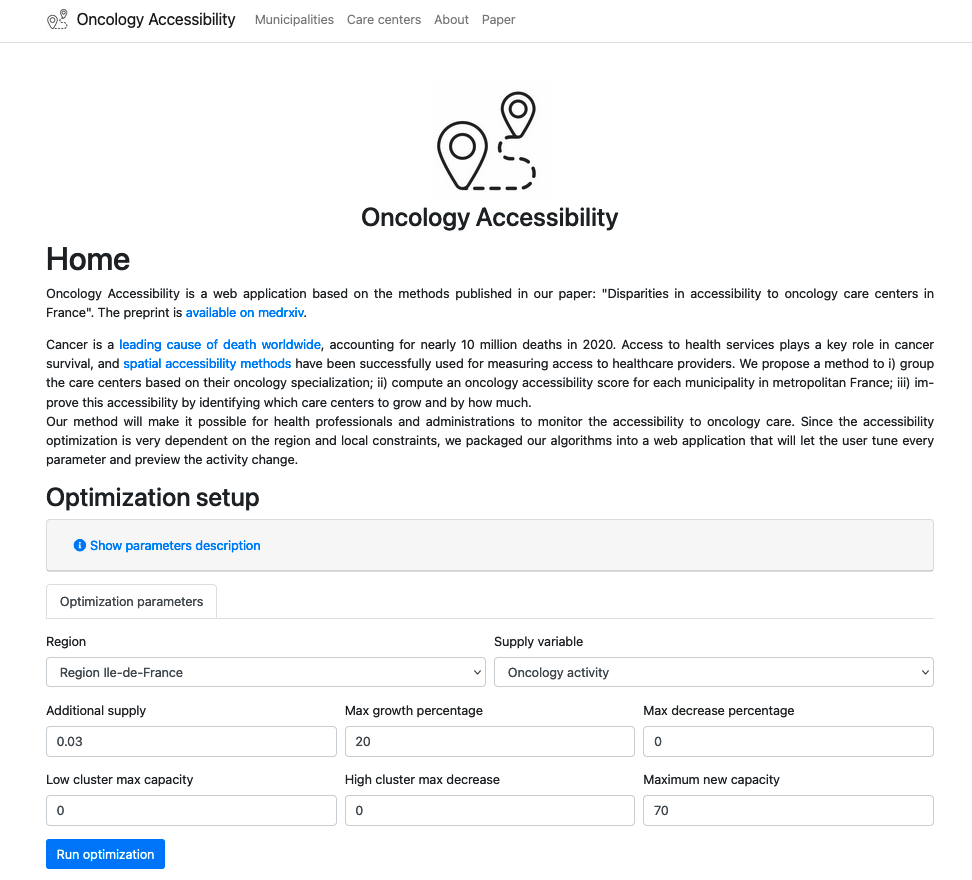
\includegraphics[width=0.9\textwidth]{images/oncology-accessibility/home.png}
    \centering
    \caption{
        \textbf{Oncology Accessibility: Homepage.}
    }
    \label{fig:optim-form}
\end{figure}

Once the parameters are set, the optimization algorithm runs and displays the
results on an interactive map, as shown on \cref{fig:optim-results}. The
accessibility delta is displayed by default on the map, as well as the hospitals
colored in green, red or green whether the hospital was grown, decreased or
remained as is. The accessibility delta is defined as the difference between the
municipality accessibility after optimization and before optimization. A
positive delta means that the municipality accessibility increased due to grown
hospitals nearby. A high delta is displayed in red on the map whereas a
municipality with a null delta is colored in pale yellow. On this interactive
map, we can also display municipalities population densities, as well as the
accessibility before and after optimization. Three histograms are placed below
the map, to compare the municipalities accessibility distribution before and
after optimization, as well as the accessibility delta distribution.

\begin{figure}[H]
    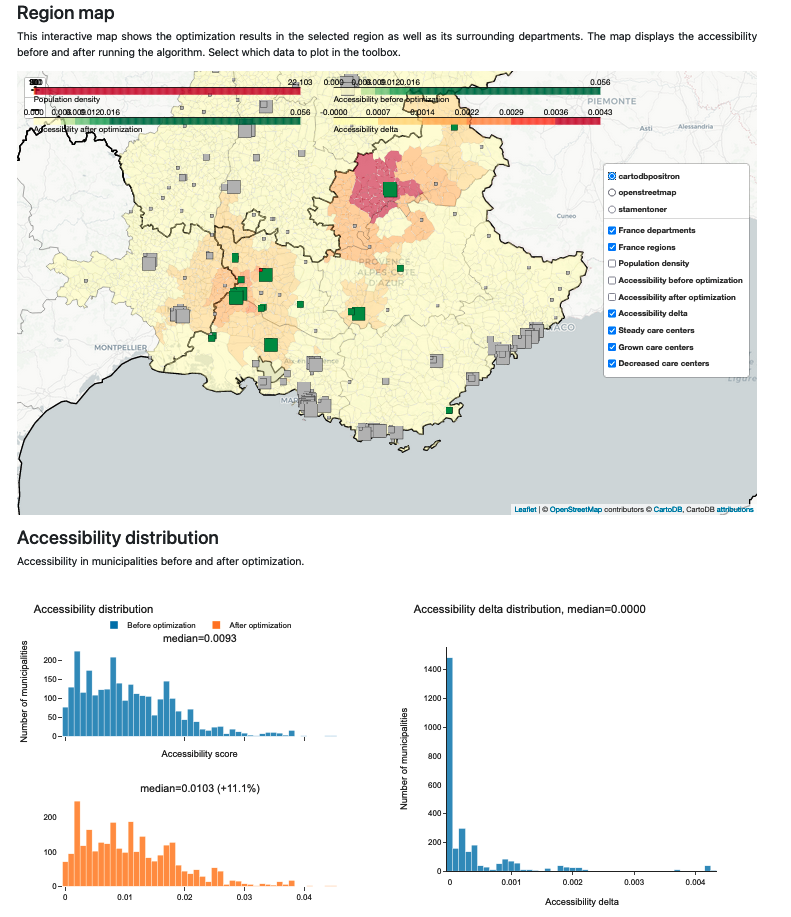
\includegraphics[width=0.9\textwidth]{images/oncology-accessibility/optim-paca-map.png}
    \centering
    \caption{ \textbf{Oncology Accessibility: Optimization results.}  The
        accessibility delta is displayed by default on the map, as well as the
        hospitals colored in green, red or green whether the hospital was grown,
        decreased or remained as is. }
    \label{fig:optim-results}
\end{figure}

Finally, the list of hospitals in the region is displayed below the histograms,
as shown on \cref{fig:optim-grown-hospitals}. The orignal capacity and modified
capacity are shown, as well as the percentage of increase. The hospital category
and cluster are displayed, for better interpretation of the modifications.

\begin{figure}[H]
    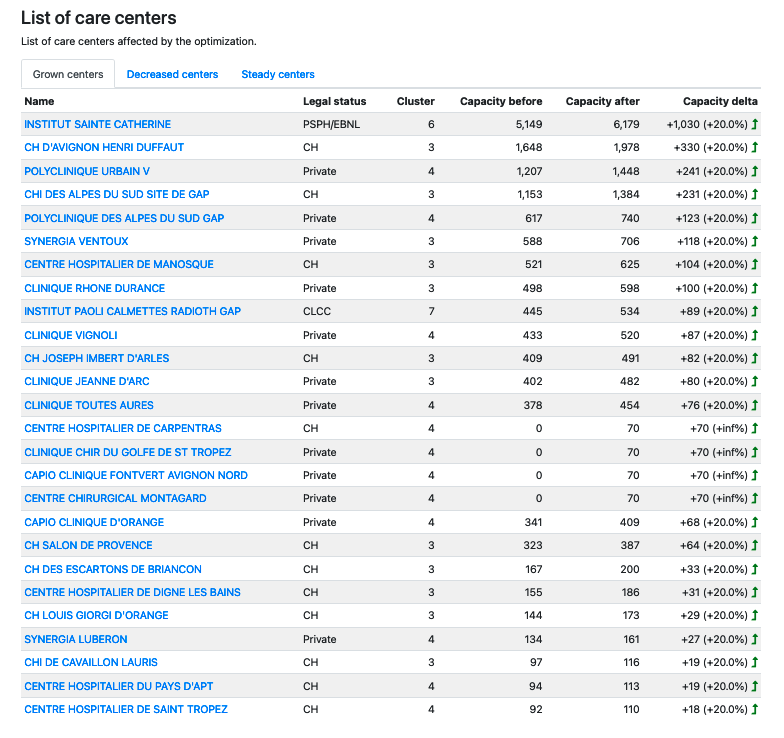
\includegraphics[width=0.9\textwidth]{images/oncology-accessibility/optim-paca-grown-hospitals.png}
    \centering
    \caption{
        \textbf{Oncology Accessibility: Optimization results.}
    }
    \label{fig:optim-grown-hospitals}
\end{figure}

On a separate web page, it is possible to get the list of municipalities and
their accessibility scores, for every region. An interactive map is also
displayed below the table, as seen on \cref{fig:optim-municipalities}.

\begin{figure}[H]
    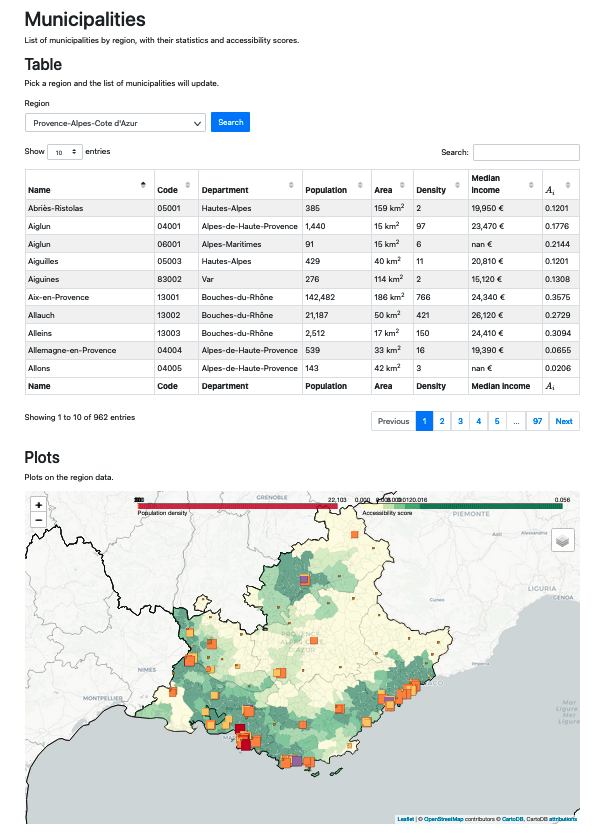
\includegraphics[width=0.9\textwidth]{images/oncology-accessibility/municipalities-paca.png}
    \centering
    \caption{
        \textbf{Oncology Accessibility: Optimization results.}
    }
    \label{fig:optim-municipalities}
\end{figure}

\section{Open source code: application on the New York City hospitals}

We open sourced the code for accessibility computation and \ac{camion}
algorithm. The code is available in the following Github repository:
\url{https://github.com/ericdaat/CAMION}. As an example to showcase our package,
we applied our method to Health Facilities in New York City. We used datasets
downloaded from NYC Open Data website, which lists free public data from New
York City agencies and other partners. We downloaded the Zip Codes boundaries
and census statistics in New York City, provided by the Department of
Information Technology and Telecommunications. We retrieved the list of health
facilities in the New York State, as well as their certifications for services
and beds. Both datasets were provided by the New York State Department of
Health. We only kept the health facilities located in New York City, with
Medical / Surgical beds. Every hospital has Latitude / Longitude coordinates. We
used Zip Codes polygons centroids as reference point to compute the travel
between Zip Codes and hospitals. We used the Zip code population as $P_i$, to
encode the demand variable. The supply variable $S_u$ was the number of Medical
/ Surgery bed for each Health Facility $u$. We used the geodesic (straight)
distance between health facilities coordinates, and Zip Code centroid
coordinates as distance matrix. The previously cited datasets can be downloaded
on the following links:
\href{https://data.beta.nyc/dataset/nyc-zip-code-tabulation-areas/resource/894e9162-871c-4552-a09c-c6915d8783fb}{Zip
    Codes boundaries and census statistics in New York City};
\href{https://health.data.ny.gov/Health/Health-Facility-General-Information/vn5v-hh5r}{List
    of health facilities in NY State};
\href{https://health.data.ny.gov/Health/Health-Facility-Certification-Information/2g9y-7kqm}{Health
    facilities certifications for services and beds}.

In the following paragraphs, we describe the hospitals in New York City and
provide code snippets to run our method. We then display the accessibility scores
and optimization results, similarly to what we did earlier for the different
regions in metropolitan France. We stress that the healthcare management is very
different in the US and in France, so we do not claim that our results should
be applied as such in New York City. We only used this dataset because it was
public, and we could easily replicate our method to show a working example to
interested users.

We first showed the spatial distribution of the included health facilities
in New York City, as seen on \cref{fig:camion-ny-beds}. Map (A) illustrates
the New York City zip codes, colored by population. The facilities are drawn
as pictograms, sized by the number of beds and colored by the county to which
they belong. The number of beds distribution is shown on histogram (B),
and the facilities with the most beds are listed on barplot (C). The largest
hospitals are mostly located in New York county.

\begin{figure}[H]
    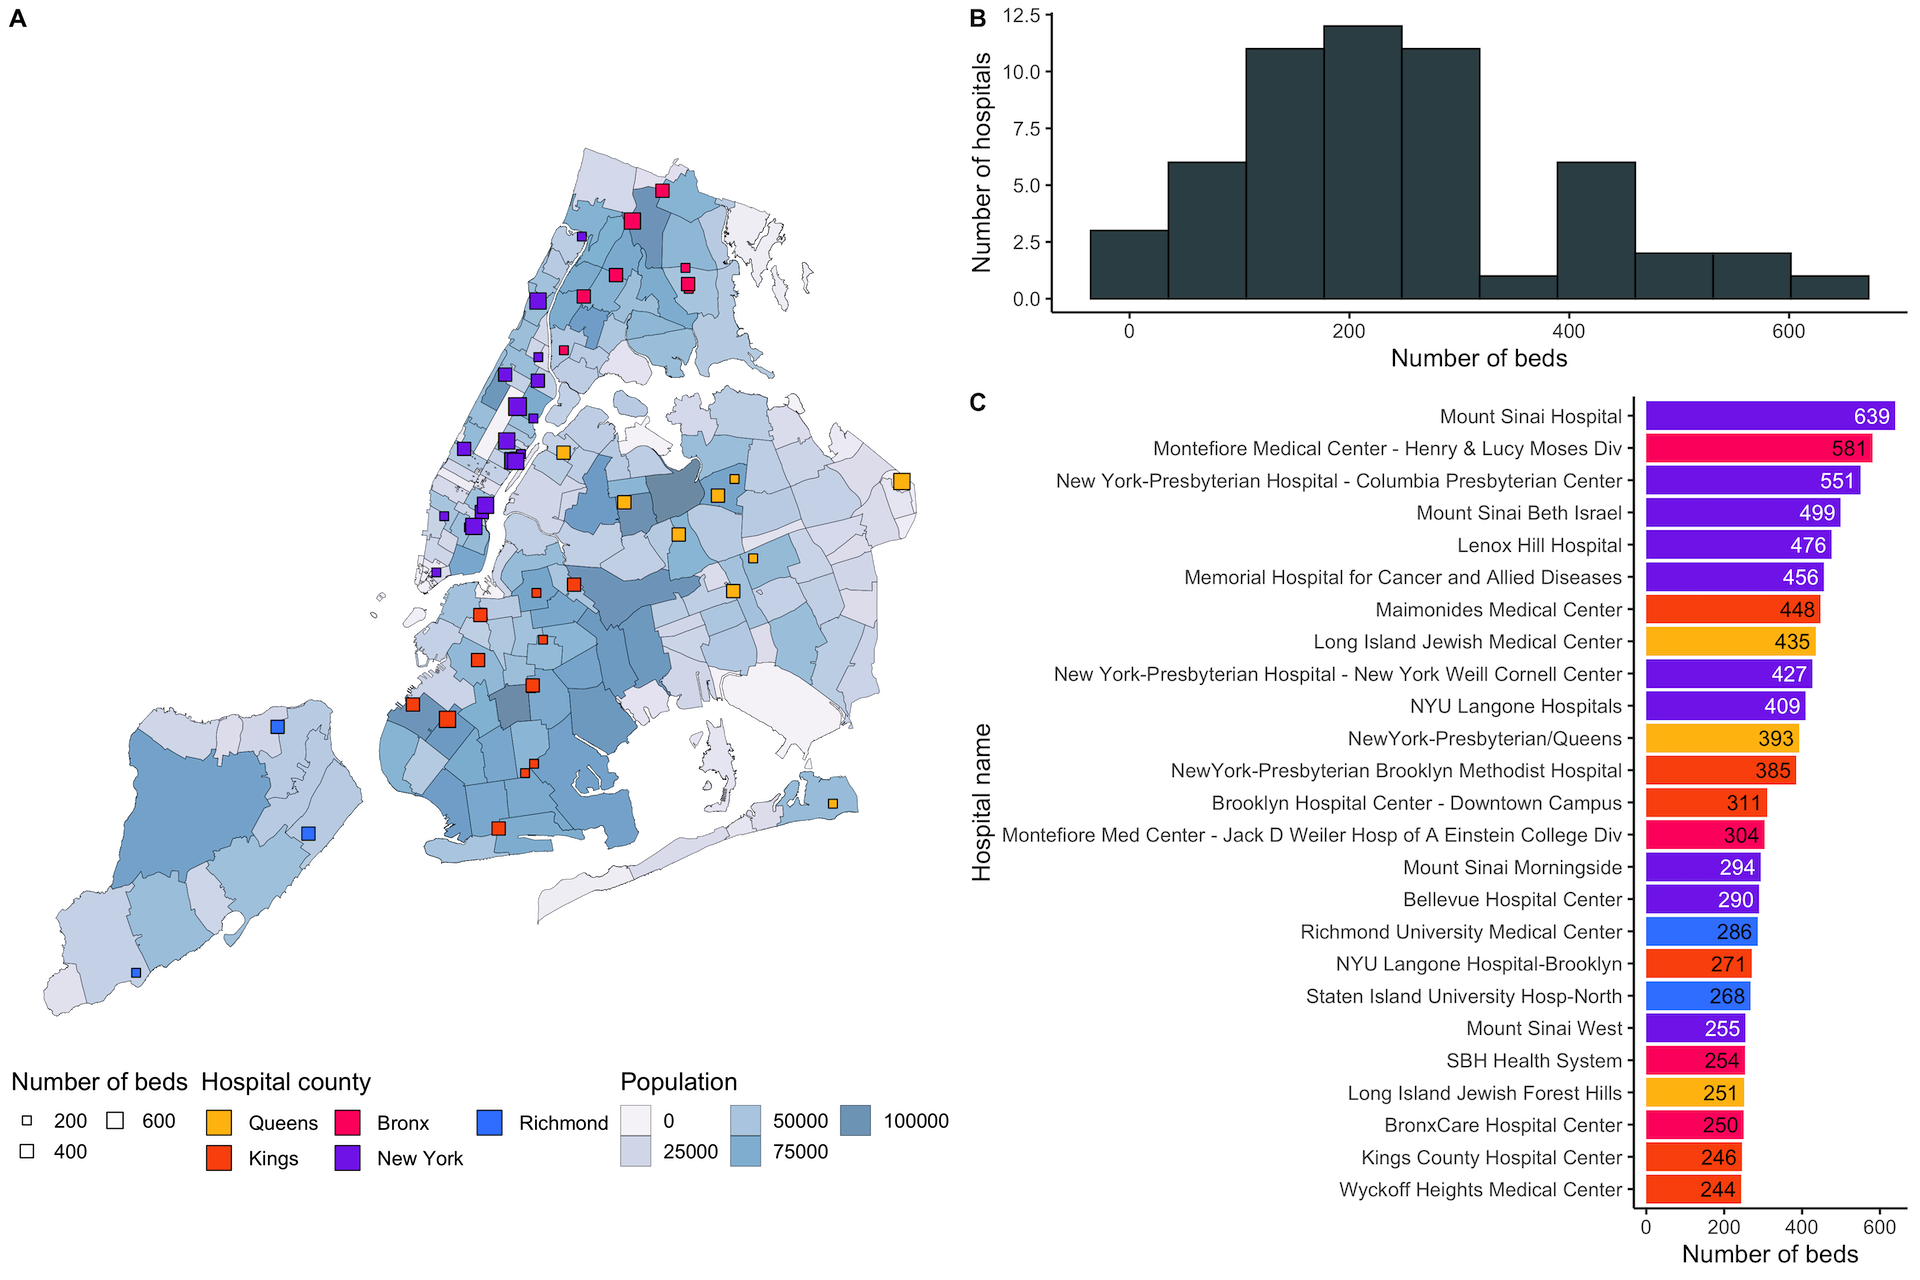
\includegraphics[width=0.9\textwidth]{images/camion-ny/fig1.png}
    \centering
    \caption{ \textbf{Health facilities with Medical / Surgery beds in New York
            City.} We included 55 facilities with a total of 13,443 beds. Map (A)
        shows the geographical location of the facilities, colored by county,
        and sized by number of beds. The distribution of the number of beds is
        shown on (B). The top 30 facilities with the highest number of beds are
        listed on (C) and colored by county. The largest facilities are in
        New-York County. }
    \label{fig:camion-ny-beds}
\end{figure}

We now show how to use our package to compute the accessibility scores with
the \ac{e2sfca} algorithm. For clarity, we used randomly generated data,
but a working example on the New York hospitals is avaiable on the Github
repository: \url{https://github.com/ericdaat/CAMION/blob/main/paper/methods.ipynb}.
For this example we sampled 100 facilities and 10 population locations. The
travel impedance were also sampled, with values between 1 and 100. The impedance
weights have been set similarly to our paper, with distance bins of 30, 60 and
90. Hence the maximum catchment area was set to 90. The following code snippet
illustrates how to initialize the data and run the algorithm.

\begin{minipage}{\textwidth}
    \begin{lstlisting}[language=Python, caption=Compute accessibility score with \ac{e2sfca}]
    from camion.fca import E2SFCA

    # Declare variables
    P_i = np.random.rand(100)  # Facilities
    S_j = np.random.rand(10)  # Population locations
    D_ij = np.random.randint(low=1, high=100, size=(100, 10))  # Travel impedance

    # Init E2SFCA algorithm
    e2sfca = E2SFCA(
        S_j=S_j,
        P_i=P_i,
        D_ij=D_ij
    )

    # Choose weights for travel impedance
    weights = [(30, 1), (60, 0.42), (90, 0.09)]

    # Compute accessibility scores
    A_i = e2sfca.compute_accessibility_score(weights)
    \end{lstlisting}
\end{minipage}

In this paragraph, we describe the accessibility results that we obtained on
the New York City dataset. The results are illustrated on
\cref{fig:camion-ny-accessibility}. The accessibility scores are displayed on
map (A) for every zip code in the city. Since the largest hospitals were located
in the New York county, it is no surprise that the highest accessibility scores
are located in that area. The Richmond county seems to have the lower accessibility
values, as shown on boxplot (C). The histogram (B) shows the accessibility
distribution. We see that the majority of the zip codes in New York City have a
high accessibility score. Finally, scatter plot (D) compares the accessibility
scores with the population for every zip code. There does not seem to be a
correlation between both series, as even zip codes with lower population
can have a good accessibility, especially in the New York county.

\begin{figure}[H]
    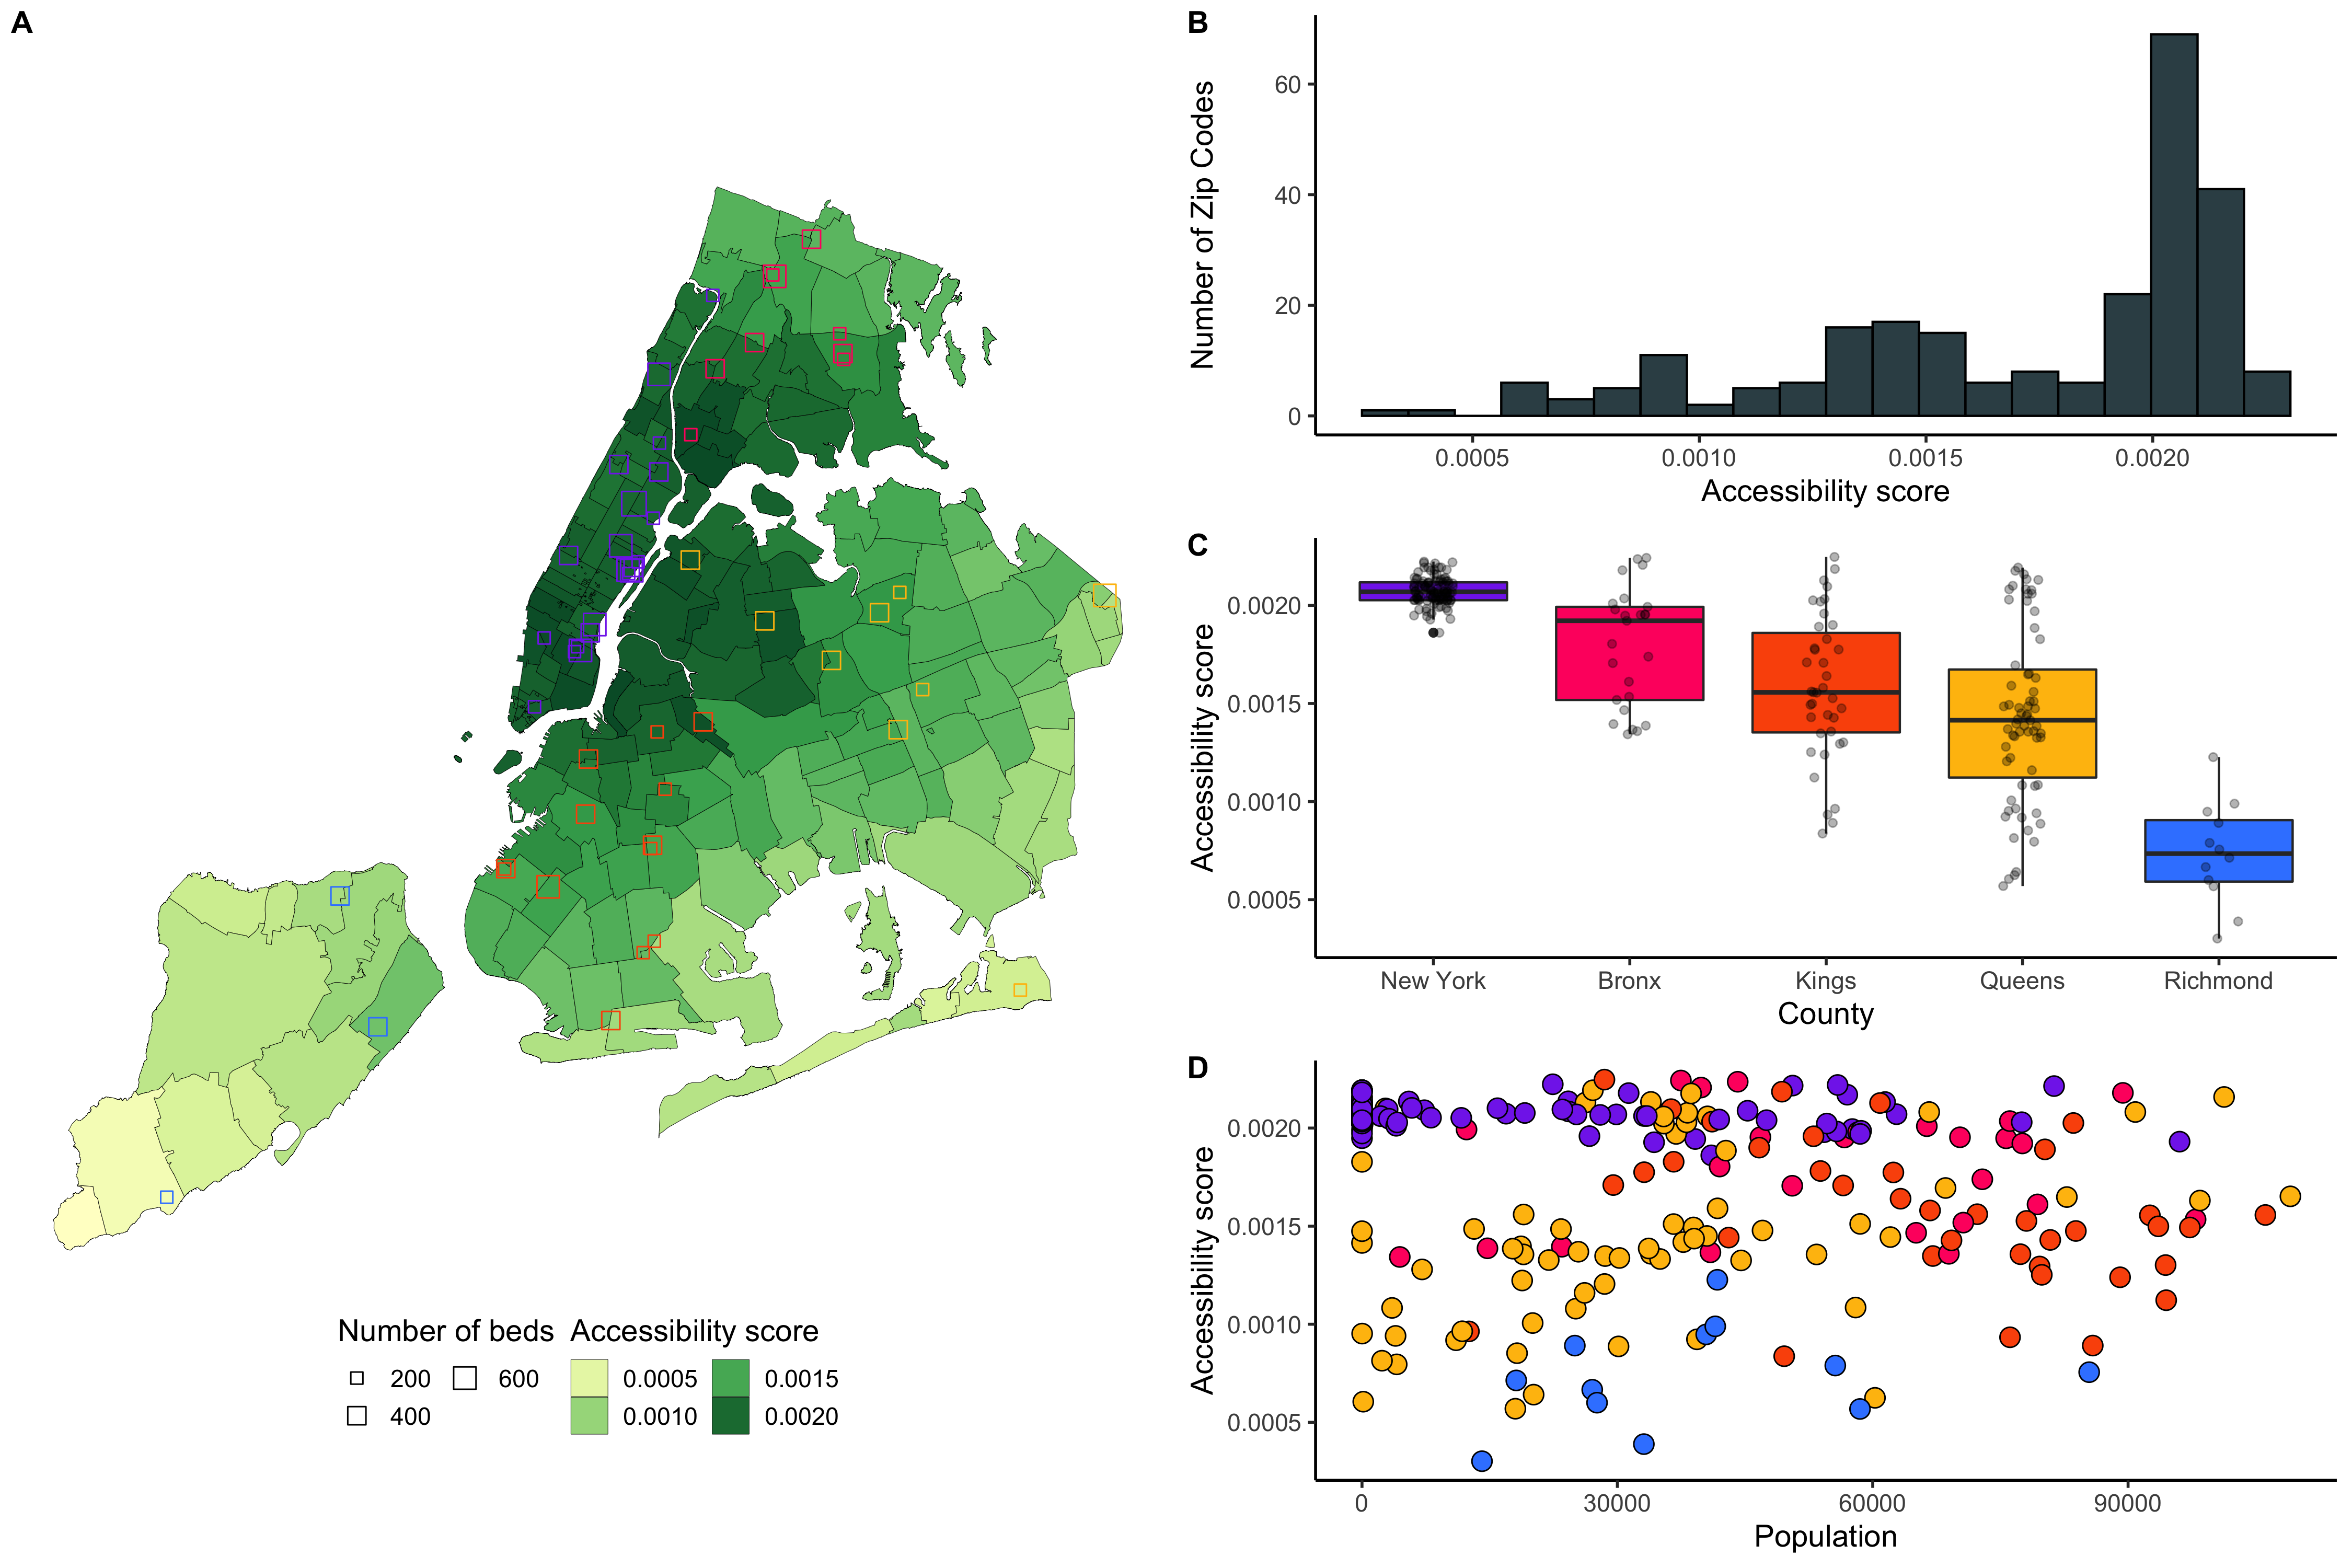
\includegraphics[width=0.9\textwidth]{images/camion-ny/fig2.png}
    \centering
    \caption{ \textbf{Accessibility to Medical / Surgery beds in New York City.}
        Accessibility score was computed with the Enhanced Two Step Floating
        Catchment Area method, with a 45 km maximum catchment area. The
        geographical distribution of the accessibility score is shown on map
        (A). Zip codes are colored by accessibility score. Facilities are sized
        by number of beds and colored by county. The overall accessibility
        distribution is shown on (B). New-York County has the highest
        accessibility distribution where Richmond has the lowest (C).
        Accessibility seems to be higher in dense areas but there is no
        significant correlation between accessibility and population (D). }
    \label{fig:camion-ny-accessibility}
\end{figure}

After computing the accessibility scores, we are now interested in running
the optimization algorithm. As we did previously, we first show a code snippet
on the previously randomly generated data, and then we display our results
obtained on the New York City dataset. In the following code snippet, we
first define the optimization parameters, namely the budget and the
maximum growth percentage for every facility. In this case, we picked a budget
of 1,000 of beds, that will be spread between the 10 facilities. The growth
percentage is set to 30\%, meaning that no facility can grow more than 30\% of
its current capacity. We then initialize the optimization algorithm, which could
either be overall optimization or maxi-min. Both methods have similar code
expressions.

\begin{minipage}{\textwidth}
    \begin{lstlisting}[language=Python, caption=Optimize accessibility with \ac{camion}]
    from camion.optimization import RegularOptimizer, MaxiMinOptimizer

    # Define optimization parameters
    budget = 1000
    growth_percentage = 0.3

    # Init regular optimizer
    regular_optimizer = RegularOptimizer()

    # Init maximin optimizer
    maximin_optimizer = MaxiMinOptimizer()

    # Run optimization with the optimization parameters
    S_j_new_regular = regular_optimizer.run_optimization(
        S_j, P_i, W_ij, budget, growth_percentage
    )
    S_j_new_maximin = maximin_optimizer.run_optimization(
        S_j, P_i, W_ij, budget, growth_percentage
    )
    \end{lstlisting}
\end{minipage}

The \cref{fig:camion-ny-optim} displays the optimization results on
the New York City dataset, using both methods, namely overall optimization (A)
and maxi-min (B). The differences between the two optimization strategies are
clearly visible. The overall optimization maximizes efficiency, thus the
algorithm focuses on areas where the population is higher, like New York or
Kings counties. On the contrary, the maxi-min approach focuses on equity,
and will address the areas with low accessibility scores first, like Richmond
county for instance.

\begin{figure}[H]
    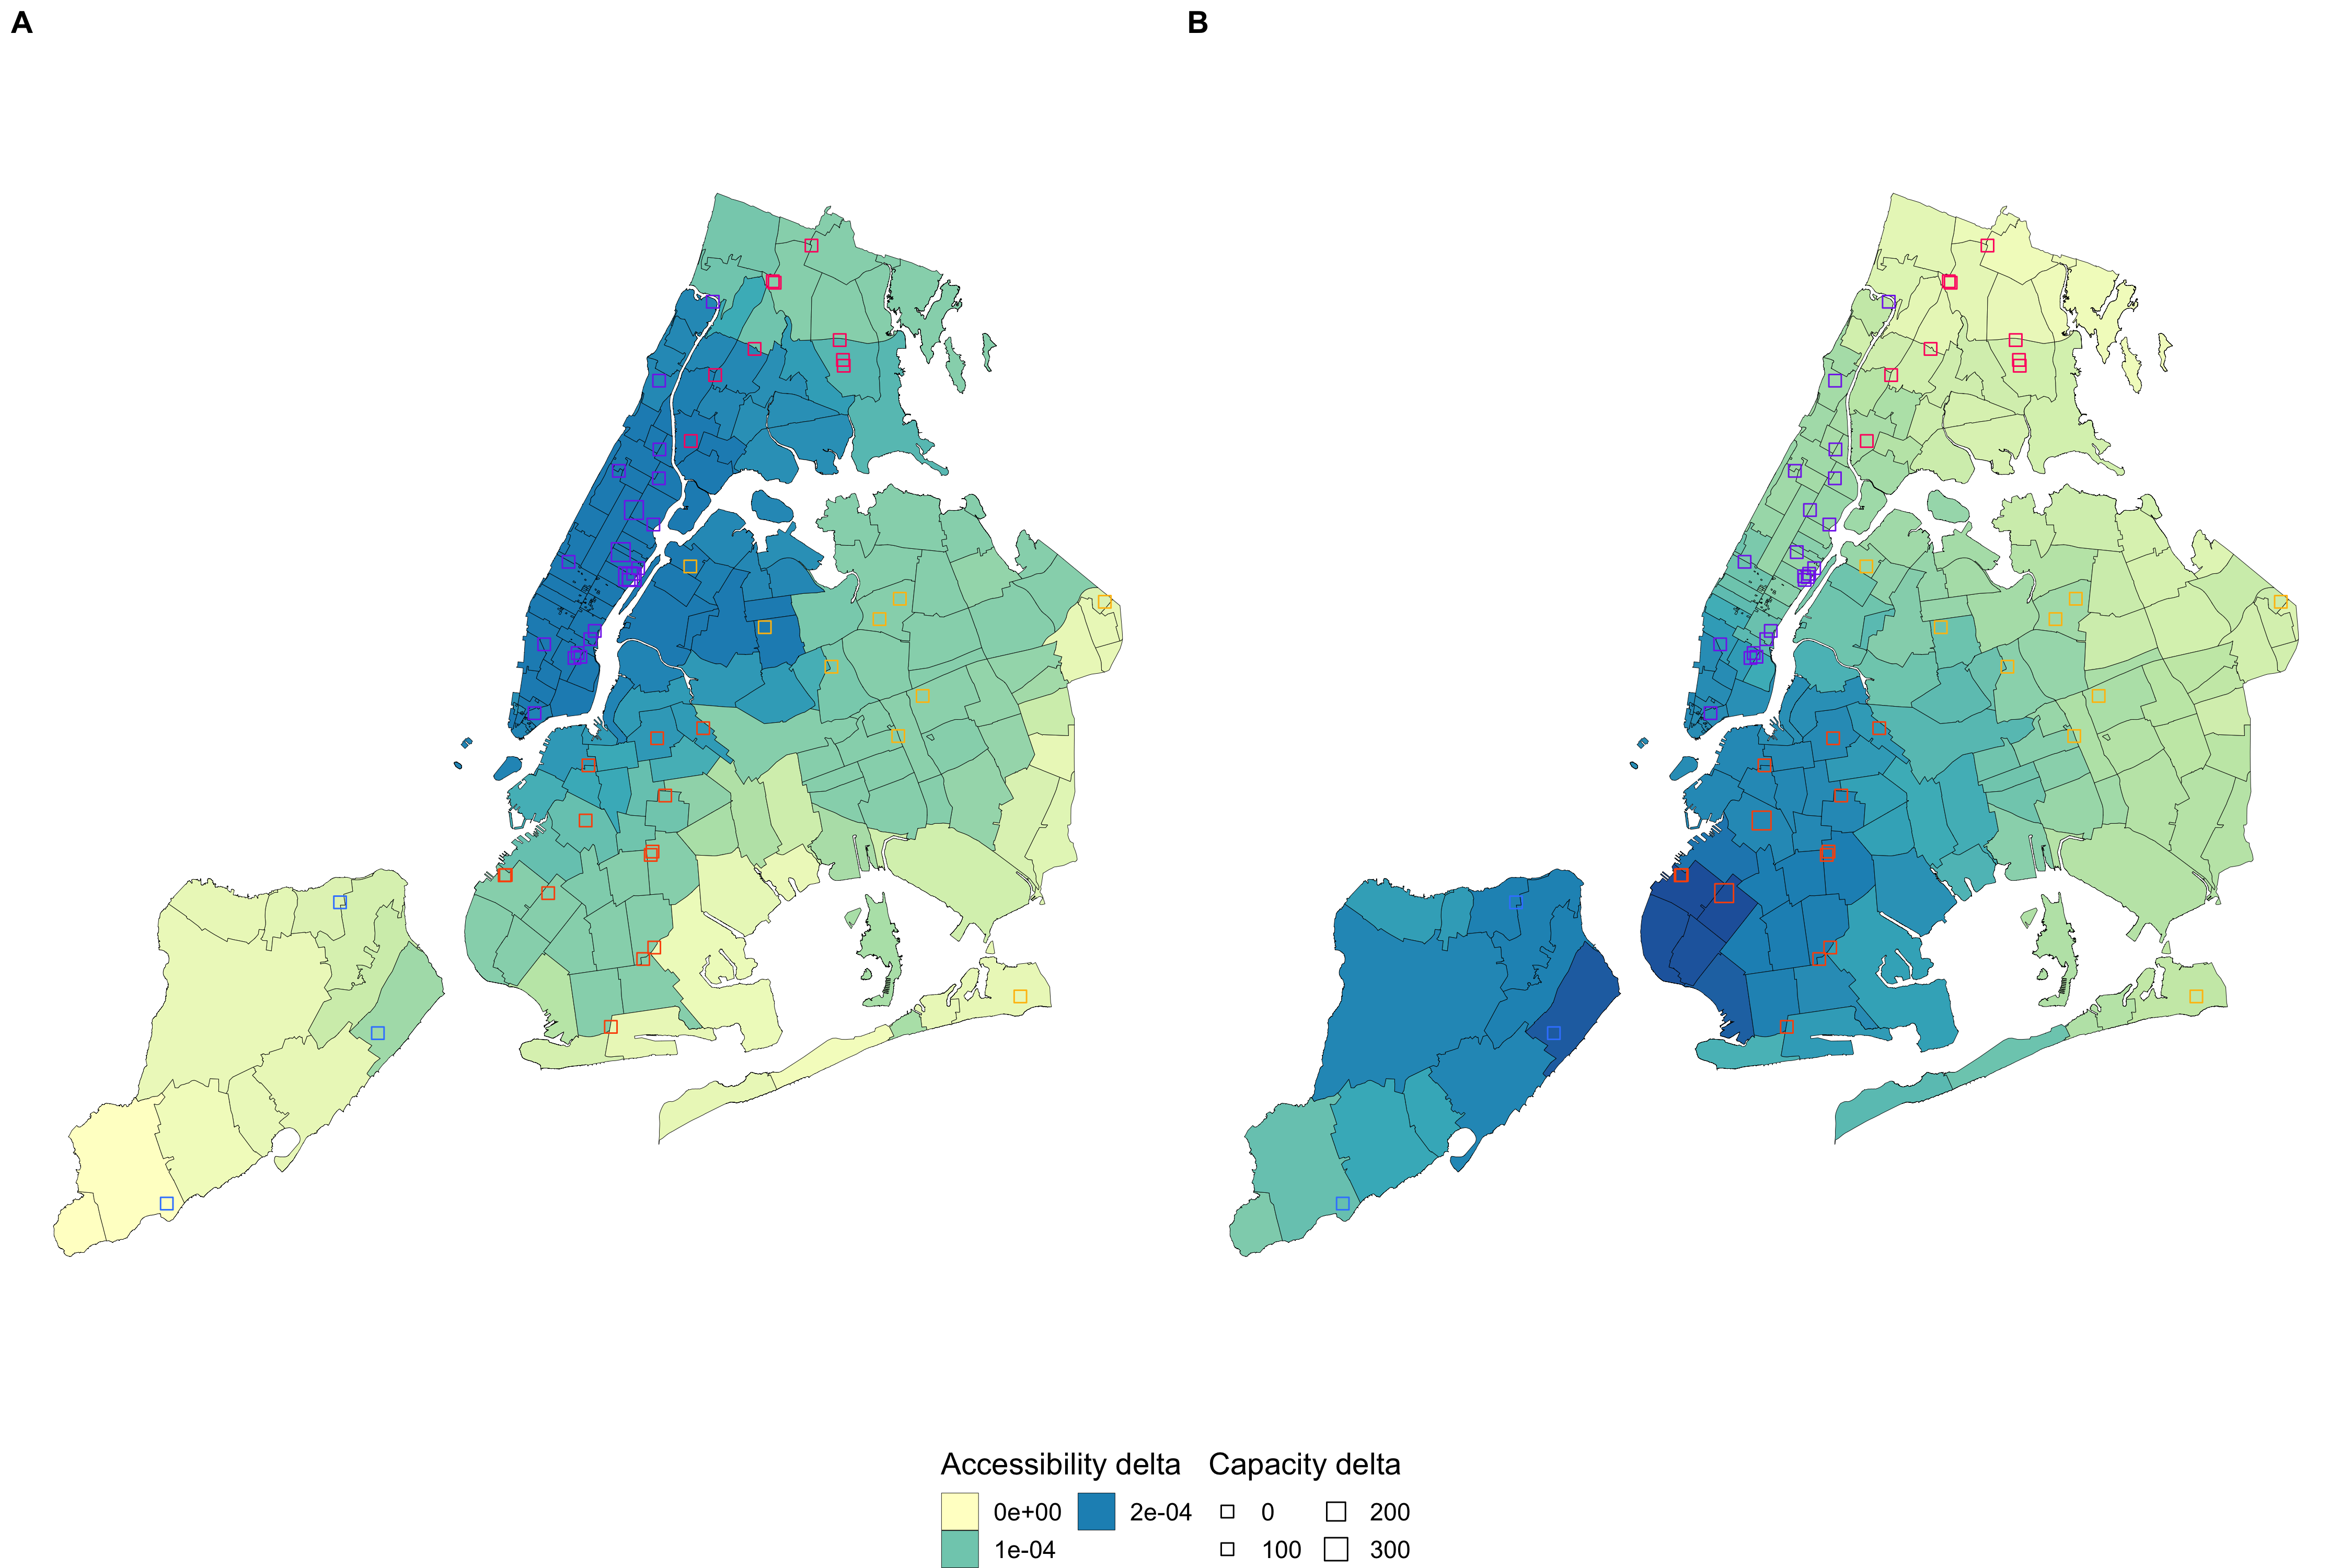
\includegraphics[width=0.9\textwidth]{images/camion-ny/fig3.png}
    \centering
    \caption{ \textbf{Accessibility delta after running the optimization
            algorithm.}Both overall and maxi-min optimization algorithms are run.
        The optimization results are illustrated on maps (A) and (B)
        respectively. We displayed the accessibility delta as the difference of
        accessibility after and before the optimization. Every zip code is
        colored by accessibility delta. The health facilities are displayed as
        squares, sized accordingly to the capacity increase. The overall
        optimization increased facilities around New-York and Queens Counties
        (A). The maxi-min algorithm targeted Richmond facilities in priority
        (B). }
    \label{fig:camion-ny-optim}
\end{figure}

\section{Conclusion}

In this chapter, we introduced CAMION, an optimization algorithm based on
\acf{lp} to optimize the accessibility distribution. The accessibility was
computed with the \acf{e2sfca} algorithm as seen previously, but our method can
generate to more Floating Catchment Area derivatives. We introduced two
optimization strategies, that either maximizes efficiency or equity in the
accessibility distribution. When we applied our method in metropolitan France,
we chose to optimize for efficiency and the optimization task was to maximize
the total accessibility instead of the minimum value. We ran the algorithm on
every region in metropolitan France and displayed the results on static maps.
However, we believe that our method could have larger benefits if the users
could run the algorithm themselves with the parameters they judge best. For this
reason, we developed ``oncology-accessibility'', a web application that embeds
our results and methods to let the users interact with our optimization
algorithm and visualize the results on interactive maps and figures. This way,
several optimization strategies could be tested to find the best approach to
reduce disparities in accessibility to oncology care in the country. Looking at
the optimization results for every region, we observed two types of optimization
outcome. For most regions, the algorithm manages to find a couple of areas where
the accessibility can be locally improved, like it did in
Provence-Alpes-Cote-d'Azur near Gap and Avignon. However, for regions like
Ile-de-France and Haut-de-France, the hospital capacity increase is more
uniformly distributed across the region. Most of the time, the algorithm left
untouched the large care centers located in dense cities with good
accessibility. This can be explained by the relatively low value of the
additional activity parameter: with a very large value of additional activity,
every care center will grow. If we keep it low, the algorithm identifies in
which areas hospital capacity should be increased in priority. The quality of
oncology care is linked with the care centers' volume. A care center with a very
low activity is less likely to provide decent care. As a result, \ac{inca}
defined several thresholds that forbid care centers with very low activity to
keep operating. Similarly, the care quality in a saturated care center won't be
good either, since patients are more likely to wait longer before diagnosis or
between interventions. While it is easy to spot care centers with low activity,
it is harder to judge if a care center is over-crowded, and we should be careful
when attributing new activity to the hospitals. We based the 20\% max growth out
of the previous centers' activity increase. This percentage could be tailored to
the center cluster or current activity. Volume is not the only factor
determining care quality. More sophisticated indicators like average delay
between diagnosis and first treatment can tell whether a care center is in line
with the care pathways recommendations. Care centers with activities lower than
the thresholds, or with a large proportion of degraded pathways should be
handled with care by our algorithm. Accessibility optimization depends on many
factors and healthcare professionals will not have the same uses for our
algorithm. Some may consider that for a care center to grow another should
decline, where others would rather not decrease any centers' activities.
Moreover, the healthcare planning is very different from a region to another,
and even within the regions departments are showing disparities. Hence, we
cannot expect the algorithm to be used with the same parameters on every region.
For all these reasons, we believe that providing a web application to run the
algorithm and choose the parameters is the most useful way to the help
healthcare professionals improve the current situation.
